%% abtex2-modelo-trabalho-academico.tex, v-1.7.1 laurocesar
%% Copyright 2012-2013 by abnTeX2 group at http://abntex2.googlecode.com/ 
%%
%% This work may be distributed and/or modified under the
%% conditions of the LaTeX Project Public License, either version 1.3
%% of this license or (at your option) any later version.
%% The latest version of this license is in
%%   http://www.latex-project.org/lppl.txt
%% and version 1.3 or later is part of all distributions of LaTeX
%% version 2005/12/01 or later.
%%
%% This work has the LPPL maintenance status `maintained'.
%% 
%% The Current Maintainer of this work is the abnTeX2 team, led
%% by Lauro César Araujo. Further information are available on 
%% http://abntex2.googlecode.com/
%%
%% This work consists of the files abntex2-modelo-trabalho-academico.tex
%% abntex2-modelo-include-comandos and abntex2-modelo-references.bib
%%

% ------------------------------------------------------------------------
% ------------------------------------------------------------------------
% abnTeX2: Modelo de Trabalho Academico (tese de doutorado, dissertacao de
% mestrado e trabalhos monograficos em geral) em conformidade com 
% ABNT NBR 14724:2011: Informacao e documentacao - Trabalhos academicos -
% Apresentacao
% ------------------------------------------------------------------------
% ------------------------------------------------------------------------

%%% TeX-command-extra-options: "-aux-directory=metafiles"
\documentclass[
	% -- opções da classe memoir --
	12pt,				% tamanho da fonte
	openright,			% capítulos começam em pág ímpar (insere página vazia caso preciso)
	twoside,			% para impressão em verso e anverso. Oposto a oneside
	a4paper,			% tamanho do papel. 
	% -- opções da classe abntex2 --
	chapter=TITLE,		% títulos de capítulos convertidos em letras maiúsculas
	%section=TITLE,		% títulos de seções convertidos em letras maiúsculas
	%subsection=TITLE,	% títulos de subseções convertidos em letras maiúsculas
	%subsubsection=TITLE,% títulos de subsubseções convertidos em letras maiúsculas
	% -- opções do pacote babel --
	english,			% idioma adicional para hifenização
	french,				% idioma adicional para hifenização
	spanish,			% idioma adicional para hifenização
	brazil,				% o último idioma é o principal do documento
	hyphens
	]{abntex2}


% ---
% PACOTES
% ---

% ---
% Pacotes fundamentais 
% ---
\usepackage{cmap}				% Mapear caracteres especiais no PDF
\usepackage{lmodern}			% Usa a fonte Latin Modern			
\usepackage[T1]{fontenc}		% Selecao de codigos de fonte.
\usepackage[utf8]{inputenc}		% Codificacao do documento (conversão automática dos acentos)
\usepackage{lastpage}			% Usado pela Ficha catalográfica
\usepackage{indentfirst}		% Indenta o primeiro parágrafo de cada seção.
\usepackage{color}				% Controle das cores
\usepackage{graphicx}			% Inclusão de gráficos
\usepackage{soul}
% ---

% ---		
% Posicionar os floats
% ---
\usepackage[bottom]{footmisc}
% http://tex.stackexchange.com/questions/62720/vertical-space-after-algorithm
% \setlength{\textfloatsep}{1.241\onelineskip}% Remove \textfloatsep
% \setlength{\floatsep}{1.241\onelineskip}% Remove \textfloatsep
% \setlength{\intextsep}{1.241\onelineskip}% Remove \textfloatsep
\setlength{\textfloatsep}{1\baselineskip}% Remove \textfloatsep
%\setlength{\floatsep}{1\baselineskip}% Remove \textfloatsep
%\setlength{\intextsep}{1\baselineskip}% Remove \textfloatsep
		
% ---
% Pacotes adicionais
% ---
\usepackage{lipsum}				% para geração de dummy text
\usepackage{siunitx}            % sistema internacional de unidades
\usepackage{amsmath,amssymb,amsthm} % pacotes matemáticos
\usepackage{pifont}             % para alguns símbolos especiais
\usepackage[version=4]{mhchem}  % fórmulas químicas
\usepackage{tabularx}
\usepackage{listings}           % para os códigos
\usepackage{multirow}           % para agrupar linhas em colunas
\usepackage{pdfpages}
% ---

\usepackage{amsthm}
\usepackage{amsmath}
\usepackage{amssymb}
\usepackage{amsbsy}
\usepackage{esint}
\usepackage{bm}
\usepackage{float}
\usepackage[most]{tcolorbox}

%---
% Pacotes de citações
% ---
\usepackage[brazilian,hyperpageref]{backref}	 % Paginas com as citações na bibl
\usepackage[alf,abnt-etal-text=it]{abntex2cite}	% Citações padrão ABNT

% --- 
% CONFIGURAÇÕES DE PACOTES
% --- 

% ---
% Configurações do pacote backref
% Usado sem a opção hyperpageref de backref
\renewcommand{\backrefpagesname}{Citado na(s) página(s):~}
% Texto padrão antes do número das páginas
\renewcommand{\backref}{}
% Define os textos da citação
\renewcommand*{\backrefalt}[4]{
	\ifcase #1 %
		Nenhuma citação no texto.%
	\or
		Citado na página #2.%
	\else
		Citado #1 vezes nas páginas #2.%
	\fi}%

\tcbset{theostyle/.style={
    enhanced,
    sharp corners,
    attach boxed title to top left={
      xshift=-1mm,
      yshift=-4mm,
      yshifttext=-1mm
    },
    top=1.5ex,
    colback=white,
    colframe=black,
    fonttitle=\bfseries,
    boxed title style={
      sharp corners,
    size=small,
    colback=black,
    colframe=black,
  } 
}}

\newtcbtheorem[number within=section]{Definition}{Definição}{%
  theostyle
}{def}

\theoremstyle{definition}
\newtheorem{definition}{Definition}
\newcommand{\R}{\bm{\mathrm{R}}}
\newcommand{\C}{\bm{\mathrm{C}}}
\newcommand{\Q}{\bm{\mathrm{Q}}}
\newcommand{\N}{\bm{\mathrm{N}}}
\newcommand{\Z}{\bm{\mathrm{Z}}}
\newcommand{\Pspace}{\bm{\mathrm{P}}}
\newcommand{\F}{\bm{\mathrm{F}}}
\newcommand{\fvec}{\bm{\mathrm{F}}}
\newcommand{\nvec}{\bm{\mathrm{n}}}
\newcommand{\vvec}{\bm{\mathrm{v}}}
\newcommand{\Svec}{\bm{\mathrm{S}}}
\newcommand{\wvec}{\bm{\mathrm{w}}}
\newcommand{\rvec}{\bm{\mathrm{r}}}
\newcommand{\xvec}{\bm{\mathrm{x}}}
\newcommand{\uvec}{\bm{\mathrm{u}}}
\newcommand{\bvec}{\bm{\mathrm{b}}}
\newcommand{\ivec}{\bm{\mathrm{i}}}
\newcommand{\jvec}{\bm{\mathrm{j}}}
\newcommand{\evec}{\bm{\mathrm{e}}}
\newcommand{\Jvec}{\bm{\mathrm{J}}}
\newcommand{\kvec}{\bm{\mathrm{k}}}
\newcommand{\zerovec}{\bm{\mathrm{zero}}}
\DeclareMathOperator{\spn}{span}

%\usepackage[margin=1cm]{geometry}
\theoremstyle{definition}
% ---

%%% -----
%%% Formato de cabeçalho/rodapé romano nos elementos pré-textuais
%%% -----

%% Novo estilo
\makepagestyle{estilo_pretextual} %%% escolha um nome
  \makeevenhead{estilo_pretextual}{}{}{\ABNTEXfontereduzida \textbf \thepage}
  \makeoddhead{estilo_pretextual}{}{}{\ABNTEXfontereduzida \textbf \thepage}

%% Customiza comando \pretextual
\renewcommand{\pretextual}{
  \pagenumbering{roman} %%% ou \pagenumbering{Roman}
  \aliaspagestyle{chapter}{estilo_pretextual}% customizing chapter pagestyle
  \pagestyle{estilo_pretextual}
  \aliaspagestyle{cleared}{empty}
  \aliaspagestyle{part}{estilo_pretextual}
}

% ---
% Ajusta a marca \textual para que a numeração volte a ser arábica
% nos elementos textuais
\let\oldtextual\textual        % copia o comando \textual anterior para \oldtextual
\renewcommand{\textual}{%
  \oldtextual%
  \pagenumbering{arabic} % volta à numeração arábica
}
% ---

% ---
% Informações de dados para CAPA e FOLHA DE ROSTO
% ---
\titulo{Uso de um modelo númerico para a otimização das curvas de secagem de concretos aluminosos}
\autor{Murilo Henrique Moreira}
\local{São Carlos -- SP}
\data{2018}
\orientador{Victor Carlos Pandolfelli}
\coorientador{Pedro Ivo Batistel Pelissari}
\instituicao{%
  Universidade Federal de São Carlos
  \par
  Centro de Ciências Exatas e de Tecnologia
  \par
  Departamento de Engenharia de Materiais}
\tipotrabalho{Trabalho de Conclusão de Curso (Graduação)}
% O preambulo deve conter o tipo do trabalho, o objetivo, 
% o nome da instituição e a área de concentração 
\preambulo{Trabalho de conclusão de curso apresentado ao curso de Engenharia de Materiais da Universidade Federal de São Carlos, como requisito parcial à obtenção do título de Bacharel em Engenharia de Materiais. Área de concentração: Cerâmicas.}
% ---

% ---
% Nova capa
% ---
\renewcommand{\imprimircapa}{%
\begin{capa}%
\center
\large\imprimirinstituicao
\par
\vspace*{3cm}
{\large\imprimirautor}\par
\vspace*{3cm}
{\ABNTEXchapterfont\bfseries\large\MakeUppercase\imprimirtitulo}
\vfill
\large\imprimirlocal
\par
\large\imprimirdata
\end{capa}
}
% ---
% Nova folha de rosto
% ---
\makeatletter
\renewcommand{\folhaderostocontent}{
\thispagestyle{empty}
\begin{center}
{\large\imprimirautor}
\vfill
{\ABNTEXchapterfont\bfseries\large\MakeUppercase\imprimirtitulo}\\
\vspace*{3cm}
\abntex@ifnotempty{\imprimirpreambulo}{%
\hspace{.45\textwidth}
\begin{minipage}{.5\textwidth}
\SingleSpacing
\imprimirpreambulo\\
\par
\imprimirorientadorRotulo~\imprimirorientador
\par
\imprimircoorientadorRotulo~\imprimircoorientador
\end{minipage}%
\vfill
}%
{\large\imprimirlocal}
\par
{\large\imprimirdata}
\end{center}
}
\makeatother
% ---

% ---
% Configurações de aparência do PDF final

% alterando o aspecto da cor azul
\definecolor{blue}{RGB}{41,5,195}

% informações do PDF
\makeatletter
\hypersetup{
     	%pagebackref=true,
		pdftitle={\@title}, 
		pdfauthor={\@author},
    	pdfsubject={\imprimirpreambulo},
	    pdfcreator={LaTeX with abnTeX2},
		pdfkeywords={abnt}{latex}{abntex}{abntex2}{trabalho acadêmico}, 
		colorlinks=true,       		% false: boxed links; true: colored links
    	linkcolor=black,          	% color of internal links
    	citecolor=black,        		% color of links to bibliography
    	filecolor=magenta,      		% color of file links
		urlcolor=blue,
		bookmarksdepth=4
}
\makeatother
% --- 

% --- 
% Espaçamentos entre linhas e parágrafos 
% --- 

% O tamanho do parágrafo é dado por:
\setlength{\parindent}{1.3cm}

% Controle do espaçamento entre um parágrafo e outro:
\setlength{\parskip}{0.2cm}  % tente também \onelineskip

% ---
% compila o indice
% ---
\makeindex
% ---

% ----
% Início do documento
% ----
\begin{document}

% Retira espaço extra obsoleto entre as frases.
\frenchspacing 

% ----------------------------------------------------------
% ELEMENTOS PRÉ-TEXTUAIS
% ----------------------------------------------------------
% \pretextual

% ---
% Capa
% ---
\imprimircapa
% ---

% ---
% Folha de rosto
% (o * indica que haverá a ficha bibliográfica)
% ---
\imprimirfolhaderosto
% ---

% ---
% Inserir a ficha bibliografica
% ---

% Isto é um exemplo de Ficha Catalográfica, ou ``Dados internacionais de
% catalogação-na-publicação''. Você pode utilizar este modelo como referência. 
% Porém, provavelmente a biblioteca da sua universidade lhe fornecerá um PDF
% com a ficha catalográfica definitiva após a defesa do trabalho. Quando estiver
% com o documento, salve-o como PDF no diretório do seu projeto e substitua todo
% o conteúdo de implementação deste arquivo pelo comando abaixo:
%
% \begin{fichacatalografica}
%     \includepdf{fig_ficha_catalografica.pdf}
% \end{fichacatalografica}
%\begin{fichacatalografica}
%	\vspace*{\fill}					% Posição vertical
%	\hrule							% Linha horizontal
%	\begin{center}					% Minipage Centralizado
%	\begin{minipage}[c]{12.5cm}		% Largura
	
%	\imprimirautor
	
%	\hspace{0.5cm} \imprimirtitulo  / \imprimirautor. --
%	\imprimirlocal, \imprimirdata-
	
%	\hspace{0.5cm} \pageref{LastPage} p. : il. (algumas color.) ; 30 cm.\\
	
%	\hspace{0.5cm} \imprimirorientadorRotulo~\imprimirorientador\\
	
%	\hspace{0.5cm}
%	\parbox[t]{\textwidth}{\imprimirtipotrabalho~--~\imprimirinstituicao,
%	\imprimirdata.}\\
	
%	\hspace{0.5cm}
%		1. Cerâmicas macroporosas.
%		2. Espumas.
%		3. Arduino.
%		I. Victor Carlos Pandolfelli.
%		II. Universidade Federal de São Carlos.
%		III. Centro de Ciências Exatas e de Tecnologia.
%		IV. Departamento de Engenharia de Materiais
%		V. Título\\ 			
	
%	\hspace{8.75cm} CDU 02:141:005.7\\
	
%	\end{minipage}
%	\end{center}
%	\hrule
%\end{fichacatalografica}
% ---

% ---
% Inserir errata
% ---
%\begin{errata}
%Elemento opcional da \citeonline[4.2.1.2]{NBR14724:2011}. Exemplo:

%\vspace{\onelineskip}

%FERRIGNO, C. R. A. \textbf{Tratamento de neoplasias ósseas apendiculares com reimplantação de enxerto ósseo autólogo autoclavado associado ao plasma rico em plaquetas}: estudo crítico na cirurgia de preservação de membro em cães. 2011. 128 f. Tese (Livre-Docência) - Faculdade de Medicina Veterinária e Zootecnia, Universidade de São Paulo, São Paulo, 2011.

%\begin{table}[htb]
%\center
%\footnotesize
%\begin{tabular}{|p{1.4cm}|p{1cm}|p{3cm}|p{3cm}|}
%  \hline
%   \textbf{Folha} & \textbf{Linha}  & \textbf{Onde se lê}  & \textbf{Leia-se}  \\
%    \hline
%    1 & 10 & auto-conclavo & autoconclavo\\
%   \hline
%\end{tabular}
%\end{table}

%\end{errata}
% ---

% ---
% Inserir folha de aprovação
% ---

% Isto é um exemplo de Folha de aprovação, elemento obrigatório da NBR
% 14724/2011 (seção 4.2.1.3). Você pode utilizar este modelo até a aprovação
% do trabalho. Após isso, substitua todo o conteúdo deste arquivo por uma
% imagem da página assinada pela banca com o comando abaixo:
%
% \includepdf{folhadeaprovacao_final.pdf}
%
% \begin{folhadeaprovacao}
% \thispagestyle{empty}
%   \begin{center}
%     {\large\imprimirautor}

%     \vfill
%     {\ABNTEXchapterfont\bfseries\large\MakeUppercase\imprimirtitulo}
%     \vfill
    
%     \hspace{.45\textwidth}
%     \begin{minipage}{.5\textwidth}
%         \imprimirpreambulo
%     \end{minipage}%
%     \vfill
%    \end{center}
    
%    Trabalho aprovado. \imprimirlocal, 28 de junho de 2018:

%    \assinatura{\textbf{\imprimirorientador}} 
%    \assinatura{\textbf{Márcio Raymundo Morelli}}
%    %\assinatura{\textbf{Professor} \\ Convidado 2}
%    %\assinatura{\textbf{Professor} \\ Convidado 3}
%    %\assinatura{\textbf{Professor} \\ Convidado 4}
    
%     \vfill  
%    \begin{center}
%     {\large\imprimirlocal}
%     \par
%     {\large\imprimirdata}
%   \end{center}
  
% \end{folhadeaprovacao}
% ---

% ---
% Dedicatória
% ---
\begin{dedicatoria}
   \vspace*{\fill}
   \centering
   \noindent
   \textit{Dedico esse trabalho aos meus pais, amigos e todos aqueles que me inspiram.} \vspace*{\fill}
\end{dedicatoria}
% ---

% ---
% Agradecimentos
% ---
\begin{agradecimentos}

Agradeço primeiramente aos meus pais, Margaret e Luiz, por todo o ensino de
responsabilidade e disciplina essenciais para alcançar meus objetivos, ao
carinho e amizade. À minha companheira e melhor amiga Mariana, pelo suporte,
atenção e ajuda em todos os momentos.

Agradeço ao Departamento de Engenharia de Materiais, pela qualidade de ensino e
inspiração que tanto professores reconhecidos proporcionam.

Ao Prof. Pandolfelli pela orientação cuidadosa ao longo de 5 anos de graduação, que sempre
auxiliou e ajudou as melhores tomadas de decisão, sendo um verdadeiro mentor e proporcionando
crescimento profissional e pessoal, estando sempre disponível para ajudar.

Agradeço especialmente ao meu coorientador, Pedro, por todos os ensinamentos,
ideias e amizade.

Agradeço também a todos do Grupo de Engenharia de Microestrutura de Materiais,
pelo suporte e parceria. Ao técnico Guilherme por estar sempre disponível.

E aos meus amigos e colegas de curso, com os quais compartilho grandes memórias,
Rodrigo, Murilo e tantos outros. 

\end{agradecimentos}
% ---

% ---
% Epígrafe
% ---
\begin{epigrafe}
    \vspace*{\fill}
	\begin{flushright}
		\textit{``Simplicidade é a conquista final.\\ Depois de uma vasta quantidade
      de notas e mais notas, \\ é a simplicidade que surge como a recompensa
      máxima da arte.''\\
		Frédéric Chopin}
	\end{flushright}
\end{epigrafe}
% ---

% ---
% RESUMOS
% ---

% resumo em português
\begin{resumo}


 \vspace{\onelineskip}
    
 \noindent
 \textbf{Palavras-chaves}: Concretos Refratários, Explosão, Modelo Numérico, FEM, FEniCS.
\end{resumo}

% resumo em inglês
\begin{resumo}[Abstract]
 \begin{otherlanguage*}{english}
 

   \vspace{\onelineskip}
 
   \noindent 
   \textbf{Key-words}: Refractory Castable, Spalling, Numerical Model, FEM, FEniCS.
   
 \end{otherlanguage*}
\end{resumo}

% resumo em francês 
%\begin{resumo}[Résumé]
% \begin{otherlanguage*}{french}
%    Il s'agit d'un résumé en français.
 
%   \vspace{\onelineskip}
 
%   \noindent
%   \textbf{Mots-clés}: latex. abntex. publication de textes.
% \end{otherlanguage*}
%\end{resumo}

% resumo em espanhol
%\begin{resumo}[Resumen]
% \begin{otherlanguage*}{spanish}
%   Este es el resumen en español.
  
%   \vspace{\onelineskip}
 
%   \noindent
%   \textbf{Palabras clave}: latex. abntex. publicación de textos.
% \end{otherlanguage*}
%\end{resumo}
% ---

% ---
% inserir lista de ilustrações
% ---
\pdfbookmark[0]{\listfigurename}{lof}
\listoffigures*
\cleardoublepage
% ---

% ---
% inserir lista de tabelas
% ---
\pdfbookmark[0]{\listtablename}{lot}
\listoftables*
\cleardoublepage
% ---

% ---
% inserir lista de abreviaturas e siglas
% ---
%\begin{siglas}
%  \item[Fig.] Area of the $i^{th}$ component
%  \item[456] Isto é um número
%  \item[123] Isto é outro número
%  \item[lauro cesar] este é o meu nome
%\end{siglas}
% ---

% ---
% inserir lista de símbolos
% ---
%\begin{simbolos}
%  \item[$ \Gamma $] Letra grega Gama
%  \item[$ \Lambda $] Lambda
%  \item[$ \zeta $] Letra grega minúscula zeta
%  \item[$ \in $] Pertence
%\end{simbolos}
% ---

% ---
% inserir o sumario
% ---
\pdfbookmark[0]{\contentsname}{toc}
\tableofcontents*
\cleardoublepage
% ---



% ----------------------------------------------------------
% ELEMENTOS TEXTUAIS
% ----------------------------------------------------------
\textual

% ----------------------------------------------------------
% Introdução
% ----------------------------------------------------------
\chapter{Introdução} \label{introducao}

\section{Apresentação do problema}
   Materiais refratários monolíticos são materiais fornecidos pelo o produtor
   sem um formato específico, podendo ter sua conformação feita pelo consumidor. Tais
   materiais apresentam inúmeras vantagens como uma maior facilidade de
   aplicação quando comparado com os materiais conformados, possibilidade de uso
   como material de reparo, e conformação de geometrias complexas.

   Porém, a etapa de queima é a principal desvantagem que essa
   categoria de materiais refratários apresenta. Tal processo exige uma queima
   lenta e cautelosa para liberar a água física e quimicamente ligada sem causar
   danos ao material. O fator de segurança para designar as curvas de
   aquecimento é comumente demasiadamente conservador, motivado pelo risco que
   uma queima má realizada apresenta de levar ao aparecimento de trincas, lascamentos e até mesmo a explosão de todo o revestimento, ou ainda, de todo o equipamento,
   conforme ilustrado na Figura \ref{fig:spalls}.
    
    \begin{figure}[ht]
        \centering
        \includegraphics[width=0.7\textwidth]{figures/spallings.pdf}
        \caption{Casos de explosão decorrente de curvas de secagem em um
          calcinador de alumina (a), no teto de um forno de alumínio (b), no
          funil de alimentação de um alto-forno (c), em um duto de gás do
          alto-forno (d). Editado de \cite{irish}}
        \label{fig:spalls}
   \end{figure}

   As dificuldades em se obter uma curva de secagem otimizada se relacionam com
   a ausência de uma metodologia que considere toda a complexidade decorrente da
   interação de diversos fatores como as condições ambientais, a geometria do
   dispositivo, o transporte de calor na peça, o transporte de massa, as
   mudanças de fase e as propriedades pertinentes em função do tempo. Sendo
   assim, o procedimento padrão se dá através da obtenção empírica das curvas de
   secagem usando comumente uma combinação de rampas e patamares conforme
   apresentado na Figura \ref{fig:hucs}.
      
    \begin{figure}[ht]
        \centering
        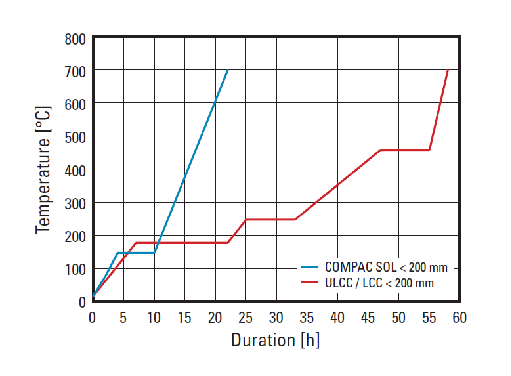
\includegraphics[width=0.7\textwidth]{figures/hucs.pdf}
        \caption{Exemplos de curvas de secagem comumente utilizadas. Retirado de \cite{rhi}}
        \label{fig:hucs}
   \end{figure}

   Portanto, o problema que o presente trabalho aborda é como usar ferramentas
   matemáticas para modelar os fenômenos de transporte de massa e calor que
   ocorrem durante a secagem para contribuir no entendimento desse complexo
   fenômeno e possibilitar que otimizações sejam realizadas tornando tal processo mais eficiente em termos de tempo e de consumo energético contribuindo para a redução dos custos financeiros e ambientais que tal processo inflige atualmente.
 
 A existência de ferramentas computacionais para a simulação de tal processo derivam de trabalhos baseados nos estudo de concretos de construção civil sujeitos a altas temperaturas em reatores nucleares ou em construções em incêndio.  Esses modelos podem considerar inúmeros processos simultâneos, o que eleva sua complexidade. Sendo assim, um desafio abordado no presente trabalho é tornar usar simplificações que possibilitem o uso de tais ferramentas em aplicações refratárias.
   
\section{Objetivos}
    \subsection{Objetivo geral}
        
    Desenvolver e implementar um modelo numérico que considere o menor número possível de parâmetros para poder prever a secagem de materiais refratários monolíticos, utilizando o ensaio de termogravimetria (TGA) para realizar a validação da simulação numérica.
        
    \subsection{Objetivos específicos}
        
    \begin{itemize}
        \item Realizar uma revisão bibliográfica sobre as metodologias de otimização de curvas de secagem;
        
        \item Desenvolver um modelo capaz de simular os resultados do ensaio de termogravimetria utilizando apenas soluções \textit{open source};
        
        \item Realizar o \textit{benchmarking} do modelo com os dados do ensaio;
        
        \item Retirar \textit{insights} do modelo e explorar casos de estudo.
    \end{itemize}
        
\section{Motivação}
   Materiais refratários são fundamentais nas principais indústrias
   habilitadoras, isto é, indústrias que fornecem maneiras de manufaturar outros
   materiais. No caso, o processo siderúrgico, que é responsável por 5 \% \cite{Davis2018} da
   liberação de CO$_2$  está intimamente relacionado com a
   indústria de materiais refratários. Tal relação é tamanha que a qualidade dos
   aços produzidos dependem diretamente da qualidade do material refratário, que
   permite, por exemplo, reduzir  o teor de carbono das ligas, por exemplo. Além disso, embora os avanços da
   área tenham reduzido consideravelmente a quantidade de refratário consumida
   por tonelada de aço (chegando até o valor de 10kgs por tonelada de aço no Japão, esse valor é ainda expressivo e com potencial para redução em diferentes mercados (como no mercado Chinês, onde estima-se um consumo de 23kgs por tonelada de aço)  \cite{refperton}.

   Nesse contexto, ampliar a vida útil dos refratários, diminuir o impacto
   ambiental de sua instalação e otimizar os tempos de manutenção podem ter
   efeitos determinantes tanto em aspectos sócio-ambientais como também
   consequências financeiras que permitam investimentos e avanços em novos
   materiais, gerando um processo contínuo de ganho de eficiência.

   A simulação do processo de secagem influencia em todos esses aspectos de
   maneira direta ou indireta, através da redução dos danos proporcionados pela
   pressão de vapor gerado no interior do material, ampliando a vida útil do
   material, agilizando a remoção da água física e quimicamente ligada, acelerando os processos de secagem e reduzindo o consumo de energia para o
   primeiro aquecimento e diminuindo as curvas iniciais de secagem, permitindo
   um ganho de eficiência no processo de manutenção dos equipamentos.

   Além dos ganhos de otimização, um maior entendimento dos processos
   concorrentes que ocorrem durante a secagem podem oferecer novos \textit{insights} para
   soluções que consigam garantir uma relação otimizada de permeabilidade e
   resistência mecânica do material, duas propriedades fundamentalmente
   inversamente proporcionais.


\section{Resultados esperados} \label{results-esperados}
   Espera-se ao final desse projeto se ter um modelo capaz de simular
   numericamente o processo de secagem de um material refratário, validado
   através de ensaios baratos (sem necessitar de inúmeros termopares e transdutores de
   pressão) com um número reduzido de parâmetros, selecionados a partir de uma
   análise de sensibilidade.

   Através do uso de tal modelo, diversos estudos de caso funcionariam como
   forma de proporcionar \textit{insights} em como otimizar o processo de secagem dos
   materiais refratários monolíticos.

    
\section{Estrutura do trabalho}
    
Esta monografia encontra-se estruturada da seguinte forma:
    
\autoref{introducao} – apresenta a introdução do trabalho, seus objetivos, motivação e os resultados esperados;
    
\autoref{fundteorica} – descreve os conceitos de materiais refratários monolíticos, apresentando suas principais características; avalia o estado da arte das metodologias de controle e otimização empírica da remoção de água de materiais refratários; apresenta modelos gerais de secagem; e por fim introduz o método dos elementos finitos, a técnica de modelamento utilizada para a resolução do modelo proposto;
    
\autoref{metodologia} – detalha os materiais e métodos utilizados no trabalho;
    
\autoref{results} – consiste na análise dos resultados obtidos tanto na caracterização das propriedades necessárias ao modelo bem como dos testes experimentais necessários para sua validação e por fim a comparação destes com os resultados numéricos discutindo-se as razões de seu funcionamento e das divergências;

\autoref{conclusao} – apresenta a conclusão do trabalho e algumas ideias para trabalhos futuros.
    
Ao final da monografia encontram-se as referências bibliográficas utilizadas, um apêndice apresentando detalhes do modelo matemático e outro contendo o programa desenvolvido na linguagem Python \cite{python}.

% ----------------------------------------------------------
% Fundamentação teórica
% ----------------------------------------------------------

\chapter{Fundamentação teórica} \label{fundteorica}
\section{Materiais Refratários Monolíticos}\label{mono}

	Os materiais refratários são componentes fundamentais nas economias modernas exercendo o papel de indústria habilitadora no sentido que possibilita a execução de processos a elevadas solicitações térmicas, químicas e mecânicas em um ambiente controlado e seguro. Ademais, o contexto sócio-ambiental do século XXI exige o máximo cuidado a fim de reduzir o desperdício de energia, especialmente de processos que ocorrem a altas temperaturas, onde a perda de energia para o ambiente é inerente.

	Assim, a indústria de materiais refratários está diretamente ligada a outras indústrias fundamentais como a indústria de cimento e principalmente a siderúrgica, ambas indústrias extremamente correlacionadas com o produto interno bruto (PIB) das nações, conforme demonstrado no gráfico temporal mostrado na Figura \ref{fig:refractory_economy}

\begin{figure}[ht]
\centering
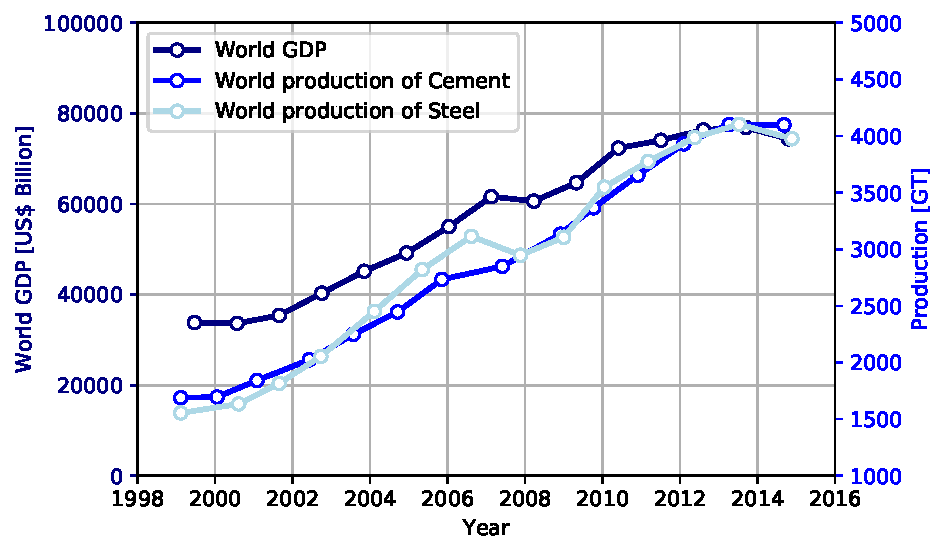
\includegraphics[width=\linewidth]{./figures/refractory_economy.pdf}
\caption{Evolução temporal do PIB mundial (azul escuro, eixo esquerdo), da produção mundial de Aço e Cimento (azul e azul claro, eixo direito) no período de 1999 a 2015.  Adaptado de \cite{GlobalRef2017}. \label{fig:refractory_economy}}
\end{figure}
		Com esse papel fundamental, os materiais refratários (que também passam por processos em alta temperatura durante sua fabricação) também passam por uma mudança de paradigma relativamente recente, isto é, ao invés do produtor fornecer peças pré-formadas (refratários conformados), este passa a oferecer um material conformável (monolítico), o que otimiza a logística - do ponto de vista do produtor, evita e reduz estoques, reduz o custo energético e permite uma maior customização do produto por parte do comprador.
        Dessarte, a seguir é realizada uma breve revisão do conceito de materiais monolíticos explorando seu processamento e finalmente vantagens e desvantagens características de tal classe de materiais.

    \subsection{Conceito}
      Capítulos 10 e 11 - Livro Ana
    

    \subsection{Processamento}
      Capítulos 10 e 11 - Livro Ana


    \subsection{Vantagens e desvantagens}
      Capítulos 10 e 11 - Livro Ana
\section{Secagem de Refratários Monolíticos}\label{secagem}
De todas as etapas de processamento de materiais monolíticos com ligantes
hidráulicos, a secagem é uma das que mais toma tempo durante o processo de
reparo [REF LIVRO]. Devido a tal fator, há um grande potencial de ganho (em
termos de tempo de reparo e energia) na utilização de procedimentos de secagem
mais eficientes. Porém, qualquer dano provocado no material durante tal etapa
compromete a vida útil do refratário.

Além de tais desafios, garantir que a secagem, de fato, siga os procedimentos
recomendados pelo produtor (as curvas de secagem) é algo complexo dado
ineficiências do sistema de aquecimento (outro setor onde a simulação
computacional pode proporcionar grandes ganhos referentes a otimização do
sistema de aquecimento, bem como maior precisão e acurácia do sistema
controlador de temperaturas) e da falta de instrução dos operadores [REF LIVRO]. Soma-se o
fato de que muitas vezes as recomendações dadas pelo produtor são motivadas muito
mais pelo temor de ter que arcar com os custos de uma explosão ou de danos ao
equipamento devido problemas na secagem do que de fato fundamentos científicos e
testes experimentais.

Sendo assim há três estratégias comuns para a redução do risco de danos durante
o processo de secagem [REF LIVRO]:

\begin{enumerate}
\item Otimização da curva de secagem: \\ Para que a maior quantidade de água
  seja removida durante o regime de evaporação e não durante o regime de ebulição;
\item Alteração da microestrutura do material: \\ Para aumentar a permeabilidade e
  diminuir o nível de pressurização no interior do material;
\item Aumento da resistência mecânica: \\ Para que o material resista às tensões
  triaxiais decorrente da pressão do vapor de água.
\end{enumerate}

As próximas seções abordam cada uma dessas estratégias de forma mais
compreensiva, de forma a mostrar o estado da arte e como as simulações
computacionais poderiam complementar os estudos nesta área.

    \subsection{Curvas de secagem}
    Uma forma bastante comum no meio industrial para se definir uma curva de
    secagem é apresentado na Figura \ref{fig:industrial_HUC}.

\begin{figure}[ht]
\centering
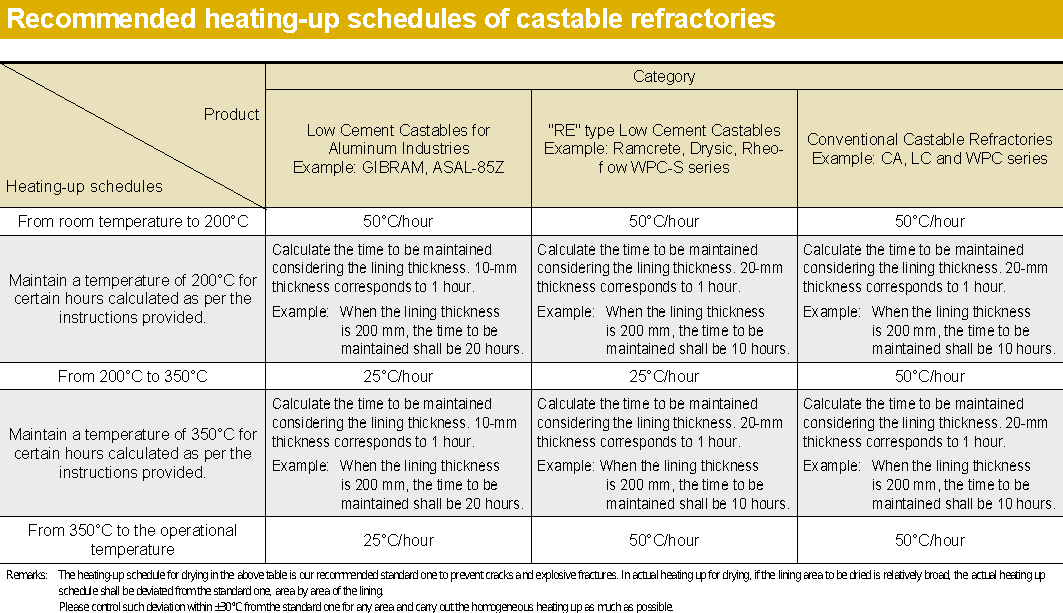
\includegraphics[width=\linewidth]{./figures/industrial_HUC.pdf}
\caption{Procedimento de secagem recomendado pela empresa AGC ceramics. Retirado de \cite{agc2016}. \label{fig:industrial_HUC}}
\end{figure}

    Observa-se que as taxas são definidas em diferentes intervalos de
    temperautra baseados aproximadamente nas temperautras de decomposição dos
    hidratos presentes no material. Além disso, o período de tempo em cada etapa
    é definido a partir da espessura do equipamento como uma maneira de se levar
    me consideração o efeito da distribuição de temperatura no interior do
    material.

    A crítica que se faz de tal procedimento é que tal correlação linear entre a
    temperatura e a espessura do componente não traduz os resultados
    experimentais e numéricos. Além disso, há a influência do próprio transporte
    de massa no interior do material nos perfis de temperatura o que pode gerar
    perfis completamente distintos.

    Tais orientações deveriam ser complementadas por resultados experimentais e
    simulações numéricas levando em conta não só as dimensões do refratário como
    também as condições de contorno, a geometria, a condutividade térmica e a
    permabilidade do material.

    Do ponto de vista empírico, ensaios de análise termogravimétrica podem ter
    grande importância para verificar se os intervalos de transofrmações
    propostos na curva de secagem, de fato correspondem com as trasnformações.

    \subsection{Aditivos para secagem}
     As recomendações 2 e 3 (alteração da microestrutura e aumento da
     resistência mecânica) podem ser implementadas através de aditivos
     adicionados na composição dos concretos. Dois casos específicos serão
     apresentados, são eles o uso de fibras poliméricas e fibras metálicas.
     Porém é importante salientar que inúmeras outras possibilidades também
     podem contribuir para o aumento de permeabilidade ou o aumento da
     resistência mecânica do material (como uso de diferentes sistemas ligantes,
     ou fases estabilizadas).

     As fibras metálicas apresentam a característica de ampliar a energia de
     fratura ao promover diferentes mecanismos de tenacificação como {\it
       crack-bridging}, {\it microcracking} e {\it pullout} [REF LIVRO]. Dessa
     maneira, há uma maior resistência ao dano por parte do material, de modo
     que as tensões devido a pressão do vapor não sejam capazes de promover o
     crescimento catastrófico das trincas. Além do efeito mecânico, o {\it
       microcracking} decorrente do {\it mismatch} dos coeficientes de expansão
     da matriz e das fibras metálicas, promove um aumento local da
     permeabilidade do material conforme reportado por Li et al \cite{li2019}.

     Por outro lado, as fibras poliméricas não apresentam quaisquer efeitos de
     tenacificação, inclusive promovendo defeitos de maiores dimenões o que
     diminui a resistêencia mecânica do material uma vez que tais polímeros são
     decompostos intencionalmente à baixas temperaturas (200$^\circ$C a
     300$^\circ$C) para promover o aumento da permeabiliade do material.

     Novamente, o uso da simulação computacional se faz importante uma vez que é
     necessário identificar a temperatura na qual a pressão no interior do
     material é máxima para selecionar o grade correto que apresente uma
     temperatura de composição coerente.

     Dessa forma justifica-se a busca por modelos númericos que possam garantir
     a otimização das curvas de secagem seja como um complemento às metodologias
     já sugeridas (como otimização da taxa de aquecimento, aumento da
     permebailidade ou aumento da resistência mecânica) ou ainda através de
     novas estratégias descobertas através da possibilidade de se obter os
     campos de pressão e temperatura no interior do material.
     
        
%%% Local Variables:
%%% mode: latex
%%% TeX-master: "TCC-Secagem"
%%% End:

\section{Modelos de Secagem}\label{modelos}
Teste 1

    \subsection{Equações de Luikov}
    Teste 2 

    
\section{Método dos Elementos Finitos (FEM)}\label{fem}
A presente seção busca introduzir alguns dos importantes conceitos referentes ao Método dos Elementos Finitos (FEM). Busca-se balancear a exposição de conceitos fundamentais com uma maneira sintética de expor tais ideias de modo a ser conciso e didático. Para mais informações refere-se a \cite{langtangen2017}, livro base onde a estrutura da presente seção foi baseada.

O procedimento padrão para a modelagem matemática de fenômenos físicos parte de Leis Fundamentais da física (como as leis de conservação de massa, $\mathcal{M}$, momento, $\mathcal{P}$, e energia interna, $\mathcal{H}$) e de propriedades características representadas por equações constitutivas (como a Lei de Hooke em elasticidade linear e a Lei de Fourier em transferência de energia térmica). O presente trabalho envolverá a resolução de um sistema de equações diferenciais parciais resultantes de duas equações de conservação (são elas, conservação de massa, $\mathcal{M}$, e de energia interna, $\mathcal{H}$) e diversas equações de estado, entre elas as curvas de sorção isotérmicas, $\phi = f(P, T)$, a Lei de Fourier para a descrição do fluxo de calor, $\vec{q}_\mathcal{H} = - k \nabla T$ e a Lei de Darcy para a descrição do fluxo de massa, $\vec{q}_\mathcal{M} = -  \frac{\kappa}{\mu} \nabla P$ (Mais detalhes em \ref{modelos}).

As equações diferenciais são os objetos matemáticos mais importantes para a
representação matemática de fenômenos físicos inclusive existindo casos de
desenvolvimentos matemáticos (em termos de terminologia e técnicas de resolução)
resultantes de inspirações obtidas nos problemas físicos referentes a cada
conjunto de equações \cite{Zauderer2006}. A descrição de taxas temporais ou de
gradientes espaciais levam em consideração a ideia do efeito que um pequeno
diferencial em uma variável independente (tempo, dimensão em $x$, $y$, ou $z$)
tem em uma variável dependente (temperatura, campo elétrico, campo magnético, tensão mecânica, etc.), com isso permitindo a descrição de fenômenos no tempo e espaço (por exemplo, como varia a temperatura $T$ em um pequeno diferencial $\partial x$).

Tais equações podem ser classificadas em equações diferencias ordinárias (ODE) quando se tem apenas funções de uma única variável independente e suas derivadas, ou em equações diferencias parciais (PDE) quando se tem funções de várias variáveis independentes e suas respectivas derivadas parciais.

No geral, as ODE's lineares podem ser resolvidas analiticamente, isto é, é
possível obter sua solução em uma forma fechada (uma expressão matemática que
pode ser avaliada em um número finito de operações algébricas). Por outro lado, as PDE's muitas vezes exigem procedimentos de solução mais complexos, fazendo uso de expansões em séries, análises de similaridade e análises assintóticas. Uma grande
complicação de tais métodos é que em geral funcionam apenas para geometrias e
condições de contorno tão simplificadas ao ponto de se distanciar
consideravelmente da realidade.

Como alternativa a tais métodos e através do avanço da capacidade computacional
os métodos numéricos alcançaram uma elevada relevância. O desenvolvimento de
\textit{softwares} comerciais permitiram que tais métodos fossem popularizados
mesmo entre usuários que não possuem conhecimento dos detalhes da implementação
de tais metodologias. Naturalmente tais \textit{softwares} se especializaram em
análises mais populares como por exemplo cálculos de análises estruturais,
análises térmicas e fluído-dinâmicas. Dessa forma, casos mais específicos onde
se tem o acoplamento de situações relativamente incomuns (como o acoplamento do
transporte de massa e de energia necessárias ao presente trabalho) não são implementados.

Assim, justifica-se o desenvolvimento de um modelo através da metodologia dos elementos finitos, uma das mais comuns metodologias de solução de PDE's e ODE's através do uso de uma malha para representar domínios com geometrias complexas. Para tanto, utilizar-se-á o pacote FEniCS da linguagem Python. Como o desenvolvimento do modelo se dará desde a escolha do tipo de elemento, das funções de forma, nós de integração entre outros, é necessário revisar os conceitos fundamentais necessários para a implementação do modelo. Também espera-se que o presente texto sirva como uma breve introdução para os alunos iniciantes nessa metodologia.

	\subsection{Métodos de aproximação de funções}
	A metodologia por trás do FEM, é uma formulação já estabelecida que permite a
  aproximação de funções de uma maneira sistemática através de funções de forma
  sobre uma malha. De uma maneira mais detalha pode-se resumir a metodologia
  como:
  \begin{enumerate}
  \item Descritização do domínio em elementos finitos
  \item Derivação de equações sobre cada elemento da malha seguindo uma
    metodologia de aproximação
  \item Acoplamento das equações locais dos elementos resultando num sistema
    global de equações lineares
  \item Imposição de condições de contorno (ajustes nas matrizes e vetores)
  \item Solução numérica das equações
  \item Pós processamento dos resultados
  \end{enumerate}

  O software FEniCS \cite{AlnaesBlechta2015a} automatiza a grande maioria das
  etapas listadas, permitindo que o foco seja nas análises dos resultados e suas
  respectivas interpretações. Assim, a presente seção não abordará aspectos
  fundamentais (como a metodologia de acoplação do sistema global ou as
  metodologias de resolução numérica do sistema) mas automatizados dando enfoque
  para aspectos que ilustrem os conceitos lógicos por trás da metodologia (como
  as metodologias de aproximação, algumas funções de elementos finitos e as
  formulações variacionais). Com  tal introdução será possível justificar a
  escolha de parâmetros do modelo como o tipo de elemento, a malha utilizada, a
  formulação utilizada entre outros.
  
  Inicialmente criaremos intuição a partir das metodologias de aproximação, em
  especial o Método de Galerkin para poder derivar as equações locais de cada
  elemento. Existem inúmeras variações de tal metodologia, com alterações
  pontuais, recebendo nomes distintos, porém no presente trabalho o uso da
  metodologia de Galerkin será o suficiente.

  Antes de introduzir a metodologia para a obtenção de soluções numéricas de equações diferenciais, iniciaremos e definiremos objetos matemáticos a partir da aproximação de Galerkin para funções (de fato funções podem ser encaradas como vetores que residem em um espaço de dimensões infinitas e portanto, a aproximação de funções se equivale à aproximação de vetores). Isso tornará a metodologia mais palpável.

  \subsection{Aproximação de Galerkin}
  Para ilustrar a metodologia utilizaremos a aproximação de uma equação trivial: 
  \begin{equation}
  \uvec = \vvec 
  \end{equation}
    Tal equação representa a busca pela melhor aproximação do vetor $\vvec$, que
    reside no espaço vetorial $V$, através do vetor $\uvec$ existente em um
    subespaço de $V$. Existem duas abordagens para encontrar o melhor vetor $\uvec$ motivadas por conceitos da álgebra linear que nos permitem formalizar algoritmos para a resolução dessa tarefa, são elas a metodologia dos mínimos quadrados e a metodologia da projeção. Tais metodologias são descritas nas Definições \ref{def:minqua} e \ref{def:metproj} .

  \begin{Definition}{Metodologia dos Mínimos Quadrados}{minqua}
  A melhor aproximação de um vetor, $\vvec$ se dá quando o vetor erro $\evec =
  \vvec - \uvec$ (isto é a diferença entre o vetor $\vvec$ e a aproximação
  $\uvec$) possui a menor norma (a partir da métrica definida no espaço vetorial
  em questão) possível, isto é: $$\frac{\partial e}{\partial c_i} = 0 $$ para
  cada coeficiente $c_i$ de cada vetor base do subespaço do espaço vetorial $V$ que abriga $\uvec$.
  \end{Definition}

  \begin{Definition}{Metodologia da Projeção}{metproj}
  A melhor aproximação de um vetor, $\vvec$, se dá quando seu erro, o vetor $\evec =
  \vvec - \uvec$ é perpendicular (o termo mais geral seria ortogonal) ao subespaço ao qual o vetor $\vvec$ reside, isto é :$$ \evec \cdot \uvec = 0 $$
  \end{Definition}
  
  A metodologia proposta na Definição \ref{def:minqua} é bastante intuitiva,
  porém a metodologia da Projeção pode ser mais complicada de se visualizar.
  Para tanto,  na Figura \ref{fig:2dvecs} é possível observar como o menor erro
  entre  $\vvec$  e  $\uvec$ se dá quando o erro  $\evec$  é perpendicular ao
  espaço onde  $\uvec$ existe.  Observe que a aproximação da figura representa a
  aproximação de dois vetores existentes em um espaço Euclidiano representado em
  coordenadas Cartesianas, o  que poderá ser generalizado para vetores definidos
  em espaços de maiores, ou ainda de infinitas dimensões. Nesse contexto, como funções são vetores, pode-se garantir que ambas metodologias acima definidas também resultarão em  metodologias de aproximação de funções (que são vetores, afinal).

  \begin{figure}[ht]
	\centering
	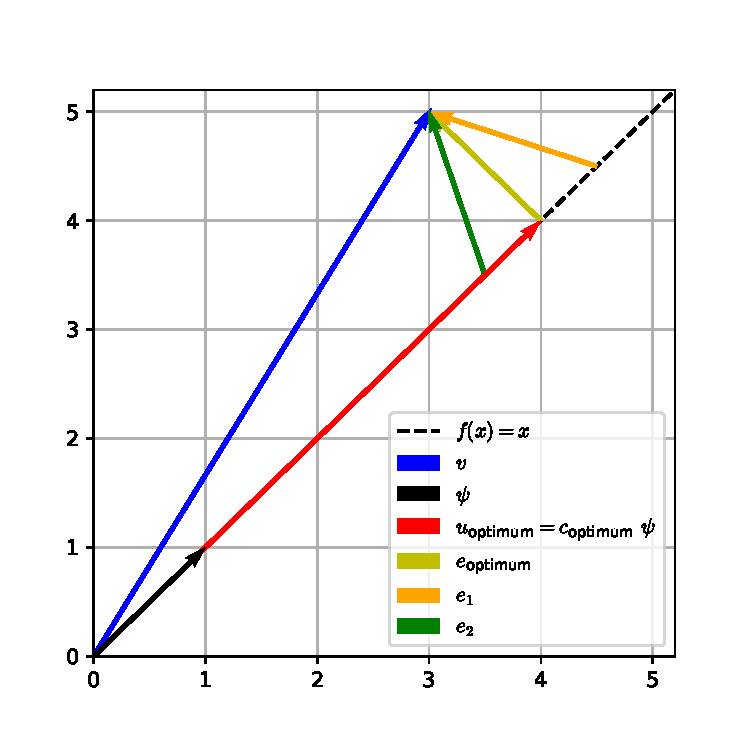
\includegraphics[width=\linewidth]{./figures/2dvectors.pdf}
	\caption{Representação da aproximação de vetores bidimensionais em coordenadas
    Cartesianas.  \label{fig:2dvecs}}
  \end{figure}

  É evidente que a melhor aproximação $\uvec_{optimum}$ resulta no erro de menor
  norma Euclidiana (comprimento do vetor, seguindo a definição de uma norma em
  um espaço vetorial Euclidiano), entretanto observe também que o erro ótimo,
  $\evec_{optimum}$ é perpendicular a reta onde reside o vetor $\uvec$ que
  estamos tentando aproximar. Lembrando-se da Geometria Analítica, quando dois
  vetores são perpendiculares seu produto interno é nulo.  

  O russo Boris Galerkin usou o mesmo  princípio para obter a solução de equações
  diferenciais, definindo o método de Galerkin \cite{reddy1993introduction}. É
  importante notar que seja na aproximação de vetores em 2D, vetores gerais ou
  funções ambas metodologias (dos mínimos quadrados e da projeção) são equivalentes.
  
	\subsection{Funções de forma}
	Como visto, anteriormente nos exemplos de vetores de duas dimensões no espaço
  Euclidiano, as aproximações de determinado vetor podem ser representadas
  através de combinações lineares de coeficientes e os vetores bases que definem
  o espaço vetorial. O que as metodologias de aproximação fornecem, são
  algoritmos que permitem encontrar o conjunto de coeficientes que formam a
  combinação linear dos vetores base cujo erro é o menor possível (dado uma certa métrica), segundo a Definição \ref{def:minqua} ou que o erro seja ortogonal ao subespaço ao qual o vetor a ser aproximado reside, segundo a Definição \ref{def:metproj}.

  	Assim, é evidente que a escolha dos vetores base é uma escolha primordial para que o processo de aproximação seja o mais prático possível. Dentre as várias possibilidades, é comum a busca por vetores ortogonais e isso pode ser mostrado pelo apelo que certas funções ortogonais apresentam como as funções trigonométricas seno e cosseno que são as bases das aproximações de Fourier.

  	No caso de tais funções trigonométricas seu domínio é o mesmo que todo o
    domínio ao qual a função a ser aproximada se estende, porém, uma estratégia
    que se pode utilizar é o uso de funções base com suporte compacto, isto é,
    funções que são não nulas apenas em uma porção do domínio, e zero em todo o
    resto do domínio, essas funções bases são as funções de elemento finito,
    usadas em FEM. A Figura \ref{fig:P1fun} ilustra uma função base de elementos
    finitos definida por partes e linear (referenciada no presente trabalho como
    $P_1$ \cite{arnold2014periodic}). Cada nó é associado com uma função desse tipo

  \begin{figure}[ht]
	\centering
	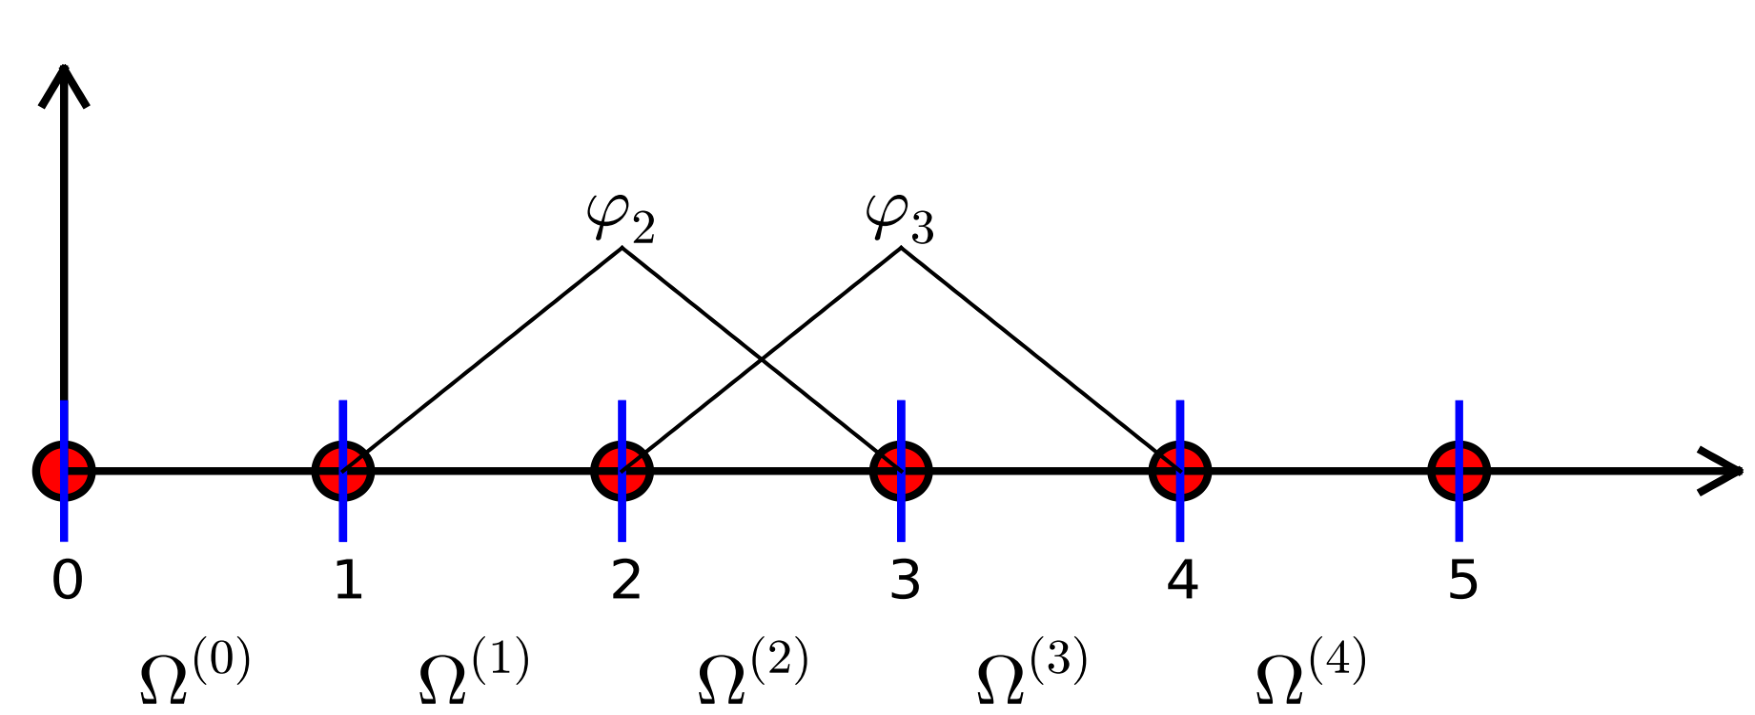
\includegraphics[width=\linewidth]{./figures/P1_fun.pdf}
	\caption{Representação de duas funções do tipo $P_1$, $\varphi_2$ e
    $\varphi_3$, em uma malha unidimensional com 5 elementos $\Omega^{(i)} $.  \label{fig:P1fun}}
  \end{figure}

  Tais funções são excelentes motivações para a divisão do domínio em uma malha,
  pois em cada elemento de determinada malha tem-se funções de forma que são não
  nulas nessa região do domínio. A vantagem é que se pode definir domínios
  complexos de uma maneira sistemática onde a convergência é obtida conforme a
  malha se torna mais refinada (isto é, com maior número de elementos
  representando o domínio) além de se obter, matrizes que são
  diagonais durante a resolução numérica o que facilita tal processo.


    \subsubsection{Malha}
    	A malha é uma partição do domínio em elementos cuja intersecção é nula e cuja união resulta exatamente no domínio. O conceito mais generalizado de um elemento finito é apresentado na Definição \ref{def:elemento}.

    \begin{Definition}{Definição Geral de Elemento Finito}{elemento}
      \begin{itemize}
        \item Um elemento finito é uma célula em um sistema de coordenadas
      locais de referência cujos limites são chamados de vértices.

        \item Em cada célula se define um conjunto de funções base do tipo de elementos
      finitos e um conjunto de graus de liberdade, isto é, quantidades que se
      busca calcular (por exemplo, a temperatura em determinado ponto ao resolver
      a equação de calor).
     
        \item Finalmente define-se um mapa entre os graus de liberdade locais (de dentro
      do elemento) e os globais (definidos em todo domínio). Tal mapa serve para
      organizar os resultados obtidos após o cálculo. Além disso, define-se um
      mapa geométrico entre a célula e o domínio físico.
      \end{itemize}
      \end{Definition}

    A princípio pode-se parecer que tais definições acabem tornando o método
    apenas mais complexo e abstrato. Porém, tal abstração garante que a
    metodologia de resolução no elemento seja feita individualmente elemento a
    elemento (inclusive usando o mesmo procedimento, pois usa-se o mesmo
    elemento de coordenadas de referência) sem considerar as especificidades
    referentes a geometria. Após o cálculo em cada elemento se realiza o
    processo de \textit{assembly} onde se une as informações de cada elemento
    obtendo os graus de liberdade em todo domínio.

    Uma vez definido a malha e os elementos a resolução do sistema de equações
    pode ser montado a partir da forma variacional do problema.

    \subsection{Forma variacional}
        Para poder utilizar o método de Galerkin o problema precisa ser reformulado
    de uma maneira específica, chamada de "Forma Fraca" ou "Forma variacional".
    Essa reformulação é o "preço" a ser pago para poder resolver um problema
    definido em um espaço com dimensões infinitas (o espaço do problema físico
    em si, definido através das leis fundamentais e equações de estado) em um
    espaço de dimensões finitas (o subespaço onde se encontrará a solução).

    Para ilustrar o conceito a subseção seguinte descreve um exemplo de
    aproximação de uma função e de uma equação diferencial.

    \subsection{Exemplos ilustrativos de aproximação de funções e equações
      diferenciais}

    
   

%%% Local Variables:
%%% mode: latex
%%% TeX-master: "TCC-Secagem"
%%% End:


% ----------------------------------------------------------
% Materiais e métodos
% ----------------------------------------------------------
\chapter{Materiais e métodos} \label{metodologia}
O presente trabalho busca propor um modelo numérico capaz de prever os perfis de
temperatura e pressão no interior de uma amostra de concreto refratário sujeito
ao aquecimento e por meio deste, otimizar uma curva de secagem. Para tanto é
fundamental o uso de experimentos para a obtenção das propriedades necessárias
ao modelo, bem como ensaios que permitam a validação do mesmo. Assim, a presente
seção apresenta o levantamento das características necessárias ao modelamento
bem como os testes para validação do modelo. Além disso, no apêncie há uma seção
específica (Apêndice \ref{codigo}) que descreve o modelo matemático bem como a
sua implementação em Python usando o pacote FEniCS. É porém de fundamental
importância determinar a composição que será utilizada e modelada, e portanto a
primeira seçaõ do presente capítulo abordará tal assunto. Ao final do capítulo o
algoritmo de controle da temperatura, capaz de otimizar a curva de secagem, será
apresentado.

\section{Composição de Concreto Refratário Aluminoso}
A composição utilizada neste projeto é de um concreto autoescoante e pode ser
encontrada na Tabela \ref{tab:composition}. Sua obtenção foi baseada no modelo
de empacotamento de Andreasen com coeficiente de empacotamento (q) igual a 0,21
\cite{da2015refractory}.

\begin{table}[]
\centering
\caption{Composição do cimento utilizado no trabalho}
\label{tab:composition}
\begin{tabular}{|l|l|l|}
  \hline
  \multicolumn{2}{|l|}{Matérias Primas}                         & Composições (wt.\%) \\ \hline
  \multirow{6}{*}{Alumina Tabular}               & AT 6-3     & 18                  \\ \cline{2-3} 
                                                                & AT 3-1     & 10                  \\ \cline{2-3} 
                                                                & AT 1-0.5   & 11                  \\ \cline{2-3} 
                                                                & AT 0.6-0.2 & 9                   \\ \cline{2-3} 
                                                                & AT 0.2-0   & 16                  \\ \cline{2-3} 
                                                                & AT<45      & 10                  \\ \hline
  \multirow{2}{*}{Alumina Calcinada e Alumina Reativa} & CL370      & 11                  \\ \cline{2-3} 
                                                                & CT3000SG   & 10                  \\ \hline
  Cimento de Aluminato de Cálcio                       & Secar 71   & 5                   \\ \hline
  Água destilada                                &            & 4.5                 \\ \hline
  Dispersante                &   Castement FS60, Basf         & 0.2                \\ \hline
\end{tabular}
\end{table}

O processamento de tal composição foi realizado através de um reômetro
especialmente desenvolvido para a preparação de concretos, no qual é possível
observar a evolução do torque nas pás do misturador, através de uma mistura
prévia da massa seca por 30 segundos e utilizando-se uma rotação de 25 rpm,
adição de aproximadamente três quartos da água até o ponto de virada (momento no
qual se dá a queda no torque mensurado) a uma rotação de 45 rpm  e adição
restante da água durante um período de mistura por 3  minutos a 55 rpm.

Em seguida os concretos foram moldados e curados em uma câmera climática à
30$^{\circ}$C por 24 horas, seguindo para as etapas de caracterização.

\section{Caracterização Experimental}\label{mat:exp}
As propriedades fundamentais para o modelo são:

\begin{itemize}
\item Permeabilidade ($\kappa$)
\item Condutividade Térmica ($\lambda$)
\item Densidade ($\rho$)
\item Calor Específico ($\C_p$)
\item Água liberada por desidratação ($w_d$)
\end{itemize}

Além disso, as curvas de sorção isotérmica também se fazem necessária, porém,
devido a ampla dificuldade em mensurá-las, o presente trabalho adotará a curva
padrão para concretos refratários reportada por Gong et al\cite{Gong1995a} e a
ajustará a mesma em caso de necessidade. Além de tais propriedades, ensaios de
Porosidade Aparente ($n_a$) e de Resistência Mecânica também foram realizados
para avaliar as suas relações com as propriedades obtidas.

\subsection{Porosidade e Densidade Aparente}\label{mat:porosidade}
A porosidade e a densidade aparente dos materiais foram obtidas através do
método de imersão usando o princípio de Arquimedes em corpos de prova tratados
previamente a temperaturas de 30$^\circ$C, 110$^\circ$C, 150$^\circ$C,
200$^\circ$C, 250$^\circ$C e 350$^\circ$C. Devido a possibilidade de hidratação
do cimento, o fluído de imersão utilizado foi querosene (conforme recomendado
pela norma ASTM C 830) e os valores de porosidade aparente, $n_a$, e de densidade
aparente, $\rho$, foram calculados conforme as Equações \ref{eq:PA} e
\ref{eq:DA}, respectivamente.

\begin{equation}
  \label{eq:PA}
  n_a (\%)= 100 \ \frac{P_u-P_s}{P_u-P_i}
\end{equation}

\begin{equation}
  \label{eq:DA}
  \rho = \frac{P_s}{P_s - P_i} \ \rho_f
\end{equation}

Onde $P_u$ é o peso a úmido, $P_i$ é o peso da amostra submerso no fluído, $P_s$
é o peso da amostra a seco e $\rho_f$ é a densidade do fluído (no caso a
densidade da querosene, $\rho_f$ = 820 Kg/m$^3$). Cada valor foi obtido através
da média de 5 amostras distintas.
    
\subsection{Permeabilidade}\label{mat:perm}

A permeabilidade dos materiais é uma medida da quantidade relativa dos poros
abertos intercomunicantes no interior de uma amostra. Para tanto, uma forma de
medi-la é através da velocidade de um fluído dado uma determinada queda de
pressão entre as faces de uma amostra. No presente modelo se faz necessário
obter a permeabilidade em diferentes temperaturas e, portanto, assume-se que
este valor pode ser aproximado pela sua medição após um
tratamento térmico em determinada temperatura, sendo a medida feita em
temperatura ambiente, seguindo a Norma ASTM C577.

As medidas são obtidas pela média dos resultados obtidos para 3 amostras de
formato cilíndrico com raio de 35mm e espessura de 25mm. Para a vedação do
sistema se utiliza silicone além de um O-ring de borracha. O esquema é
apresentado na Figura \ref{fig:perm}. O modelo utiliza a permeabilidade
hidráulica que é obtida a partir da constante de permeabilidade Darciana
($k_1$), que representa as perdas de energia viscosa a baixas velocidades do ar.
A medida de permeabilidade realizada também permite a obtenção do parâmetro
$k_2$ devido a não linearidade da velocidade, caracterizada pela equação de
Forchheimer, \ref{eq:forch}. Este segundo parâmetro diz respeito a perda de
energia cinética a altas velocidades.

\begin{equation}
  \label{eq:forch}
  \frac{P_e^2 - P_s^2}{2 \ P \ L} = \frac{\mu}{k_1} \ v_s + \frac{\rho}{k_2}v_s^2
\end{equation}

Onde $P_e$ e $P_s$ são as pressões absolutas na entrada e na saída da amostra
medidas em atm, $P$ é a pressão a uma determinada vazão de ar, $L$ é a espessura
da amostra em mm, $\mu$ é a viscosidade do ar medida em Pa s, $\rho$ é a
densidade do ar g/cm$^3$ e $v_s$ é a velocidade do fluído em m/s.

\begin{figure}[ht]
	\centering
	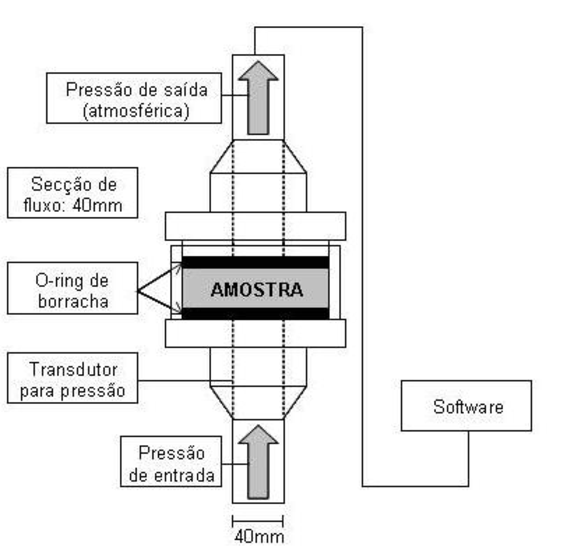
\includegraphics[width=9cm]{./figures/perm.pdf}
	\caption{Esquema de montagem do ensaio da medida de
    permeabilidade. \label{fig:perm}}
\end{figure}

   

\subsection{Resistência Mecânica}\label{mat:rm}
A resistência mecânica foi obtida através do ensaio de flexão em 3 pontos no
mesmo intervalo de temperaturas usado para a obtenção da porosidade e densidade
aparente, sendo realizados de acordo com a norma ASTM C133 utilizando 5 corpos
de prova no formato de paralelepípedos com dimensões de 25 x 25 x 150 mm$^3$. O
equipamento utilizado foi uma máquina de ensaios mecânicos universal (MTS,
Modelo 810, USA) usando uma taxa de carregamento constante de 12.9 N.s$^{-1}$. O
módulo de ruptura ($\sigma_f$) foi calculado pela Equação \ref{eq:modulo_rup}.

\begin{equation}
  \label{eq:modulo_rup}
  \sigma_f = \frac{3 \ P \ L}{2 \ b \ d^2}
\end{equation}

Onde $P$, é a carga de ruptura medida em N, L é a distância entre os apoios,
fixa em 127 mm; b é a largura e d, a altura do corpo de prova em mm.
    
\subsection{Termogravimetria (TGA)}\label{mat:TGA}

Ensaios termogravimétricos são as principais ferramentas usadas para a simulação
do processo de explosão de corpos cerâmicos em escala laboratoriala. O sistema
utilizado neste projeto consiste em um forno com uma balança acoplada, onde se
mede a temperatura da amostra e do forno, além da evolução do peso de uma
amostra cilíndrica com 50 mm de diâmetro e 50 mm de altura. Os corpos são
aquecidos após cura a 30$^\circ$C por 24 horas. Foram utilizadas taxas de
aquecimento constantes de 2$^\circ$C.min$^{-1}$, 5$^\circ$C.min$^{-1}$ e
20$^\circ$C.min$^{-1}$ no intervalo de 30$^\circ$C e 800$^\circ$C. A perda de
massa e sua taxa foram obtidas através das Equações \ref{eq:TGA_W} e
\ref{eq:TGA_DTG}.

\begin{equation}
  \label{eq:TGA_W}
  W = \left( \frac{M_0-M}{M_0-M_f} \right) \ 100
\end{equation}

\begin{equation}
  \label{eq:TGA_DTG}
  DTG = \frac{\partial W}{\partial t}
\end{equation}

Onde $M_0$ é a massa inicial da amostra, $M$ é a massa observada num instante t,
e $M_f$ corresponde à massa final da amostra (todas medidas em gramas). $W$ é a
perda de massa percentual, enquanto DTG é a taxa de perda de massa (medida em
\%.min$^{-1}$). A Figura \ref{fig:TGA} apresenta o esquema de montagem do ensaio
de termogravimetria.
    
\begin{figure}[ht]
	\centering
	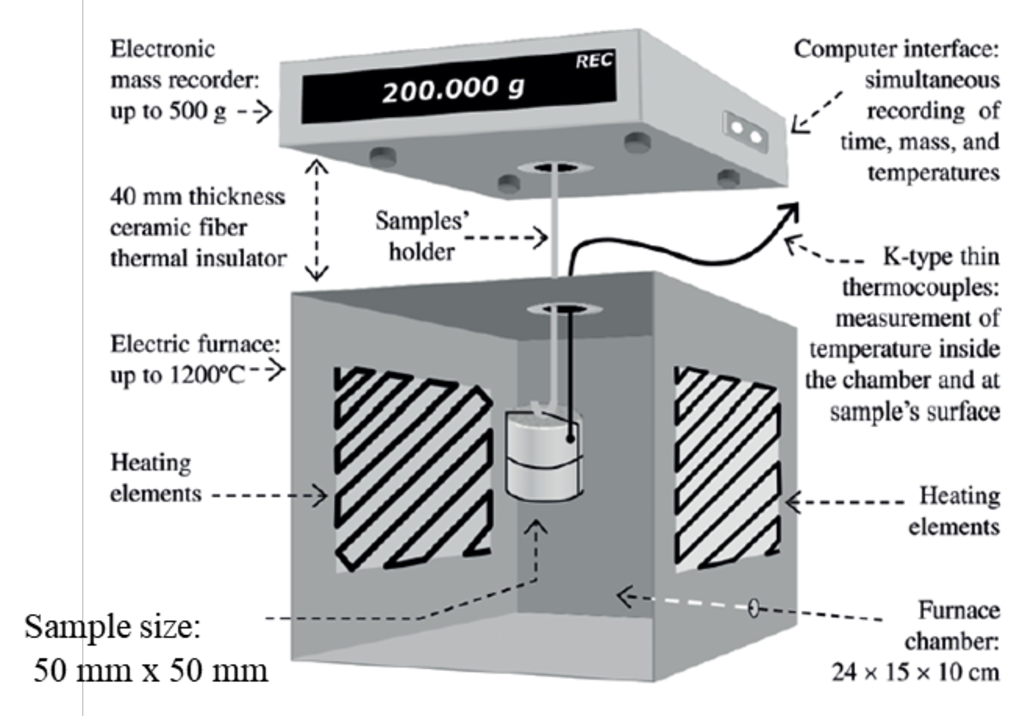
\includegraphics[width=9cm]{./figures/TGA.pdf}
	\caption{Esquema de montagem do ensaio de termogravimetria. \label{fig:TGA}}
\end{figure}



\subsection{Condutividade Térmica e Calor Específico}\label{mat:condutividade}
A condutividade térmica é obtida através do método do fio quente (com a
configuração dos fios paralelos) através do equipamento Netzsch TCT 426. A
medição se dá em um sistema de 3 tijolos com mesma composição dispostos um sobre
os outros. Entalhes de 0.4mm são realizados nos tijolos usando uma retífica
modelo Ferdimat T42 a fim de acomodar os fios do termopar.

A técnica obtém o valor de condutividade através de uma estimativa baseada no
tempo em que o calor gerado pelo fio quente (FQ), devido ao efeito Joule, leva
para ser percebido no termopar da amostra ($T_a$) em uma condição de equilíbrio
térmico entre o conjunto de tijolos e o forno (através da medida de um termopar
de referência $T_r$). Tal ensaio permite a obtenção do calor específico através
da medida de difusividade térmica do material. A Figura \ref{fig:fio_quente}
apresenta o {\it layout} do ensaio.

\begin{figure}[!ht]
	\centering
	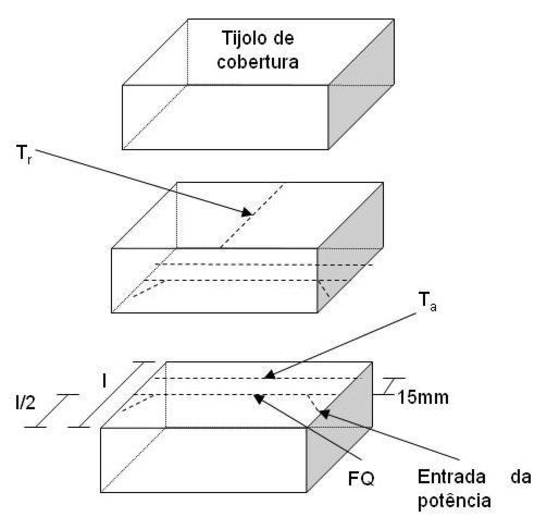
\includegraphics[width=9cm]{./figures/fio_quente.pdf}
	\caption{Esquema de montagem do ensaio da técnica de fio quente para obtenção
    da condutividade térmica e calor específico. \label{fig:fio_quente}}
\end{figure}

\section{Algoritmo de Otimização das Curvas de Secagem}\label{mat:pid}
A estratégia para obtenção de curvas de secagem otimizadas assemelha-se à
abordagem adotada por Fey et al \cite{Fey2017c}, na qual um controlador PID é
utilizado para controlar a temperatura a partir da pressão nos poros do
material. Assim, a abordagem em si não é baseada em um algoritmo de otimização,
no sentido no qual não se buscará encontrar os parâmetros que definem uma curva
de secagem de um ótimo local ou global, mas sim buscará ter-se o controle da
pressão, evitando que seus níveis alcancem a resistência mecânica do material, o
que levaria a trincas ou explosões. O algoritmo funciona a partir do cálculo de
um erro $e$ entre a pressão máxima no interior dos poros do material,
$P_v^{max}$ , e a pressão máxima permitida $P_{max}$. Tal erro dependerá do
tempo e será recalculado em cada passo de tempo, conforme a Equação
\ref{eq:erro_pid}.

\begin{equation}
  \label{eq:erro_pid}
  e(t) = P_v^{max} - P_{max}
\end{equation}

Uma vez calculado o erro, é obtido a taxa de aquecimento instantânea (constante
naquele passo de tempo) ao qual a amostra será submetida, calculada segundo a
Equação \ref{eq:T_Rate}.

\begin{equation}
  \label{eq:T_Rate}
  \Delta T = K_{p} e(t)+K_{i} \int_{0}^{t} e(\tau) d \tau+K_{d} \frac{d e(t)}{d t}
\end{equation}

Uma das mais difíceis etapas para o uso de controladores PID é a definição das
constantes dos termos proporcional, integral e derivativo \cite{ogata2002}. No
presente trabalho, o refinamento de tais coeficientes foi realizado manualmente,
sendo $K_p = - 2.00 \ 10^{-6}$, $K_i= -6.25 \ 10^{-8}$ e $K_d = 0.00$, ou seja,
o termo derivativo utilizado é nulo, pois do contrário, as oscilações observadas
na variável de resposta eram muito elevadas.
 
  
%%% Local Variables:
%%% mode: latex
%%% TeX-command-extra-options: "-shell-escape"
%%% TeX-master: "TCC-Secagem"
%%% End:


% ----------------------------------------------------------
% Resultados e discussão
% ----------------------------------------------------------

\chapter{Resultados e discussão} \label{results}
\section{Propriedades}
As propriedades do material necessários para a simulação são a condutividade
térmica, o calor específico, a densidade, a permeabilidade e a água quimicamente
ligada, conforme apresentadas na Figura \ref{fig:properties}.

 \begin{figure}[ht]
\centering
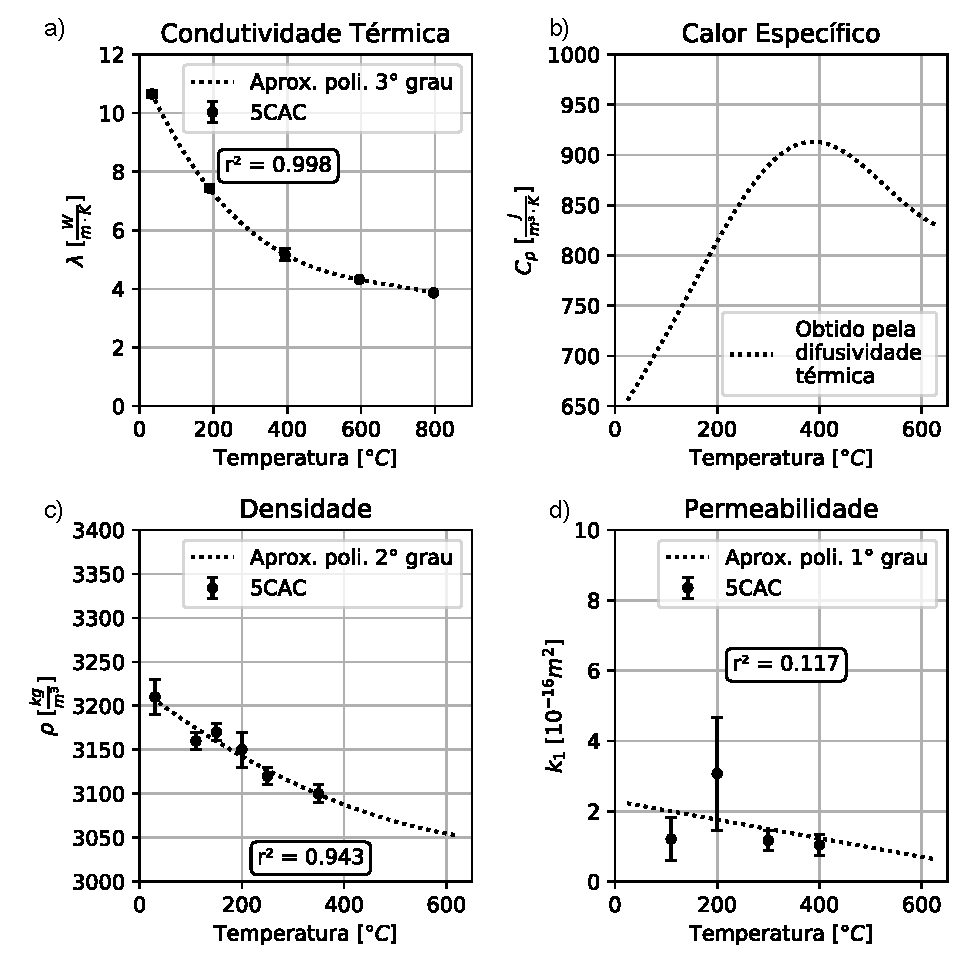
\includegraphics[width=14cm]{./figures/properties.pdf}
\caption{Caracterização da composição de concreto refratário utilizado no
  presente estudo, (a) condutividade térmica, (b) calor espicífico, (c)
  densidade e permeabilidade (d).  \label{fig:properties}}
\end{figure}

A condutividade térmica decaí conforme a temperatura aumenta. Tal comportamento
pode ser aproximado por um polinômio de terceiro grau. Este comportamento
justifica-se pelo aumento da frequência de oscilações dos átomos, o que diminui
o caminho livre médio dos fónons que são os principais transportadores de
energia térmica até aproximadamente 800$^\degree$C quando o transporte por
radiação começa a predominar \cite{pelissari2017}. A densidade é reduzida devido
a liberação da água físicamente adsorvida, bem como a água quimicamente ligada.
Outro efeito provável é a conversão de fases menos densas do cimento aluminoso
hidratado em fases de maior densidade, o que amplia a porosidade do material. O
calor específico foi calculado a partir da medida de difusividade térmica,
$\alpha = \frac{\lambda}{\rho \ C_p}$, e portanto não é apresentado o desvio
associado. Por fim, a permeabilidade do material apresenta um desvio padrão
muito elevado, e isto reflete no baixo valor de $r^2$ (aqui uma possível solução
seria aumntar o grau do polinômio, porém, seria o equivalente a realizar um {\it
  overfitting} uma vez que estaríamos inserindo no modelo um comportamento que
pode ser apenas o produto do erro da medida \cite{raschka2017}). 

 \begin{figure}[ht]
\centering
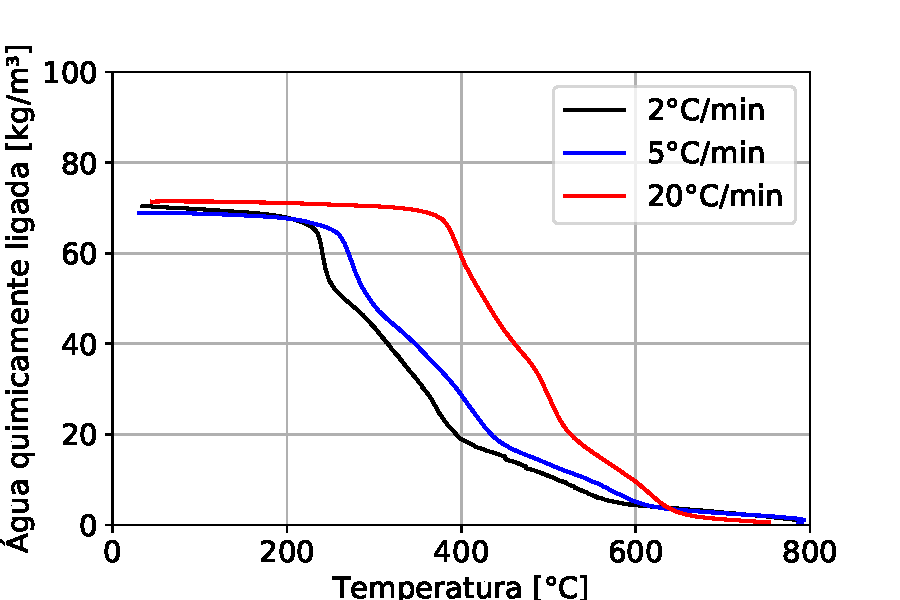
\includegraphics[width=14cm]{./figures/w_d.pdf}
\caption{Água quimicamente ligada por $m^3$ de concreto.  \label{fig:prop_wd}}
\end{figure}

Na Figura \ref{fig:prop_wd} a curva de liberação de água químicamente ligada é
apresentada. Sua medição é realizada a partir do ensaio de TGA realizado em
amostras previamente secas à 110$^\degree$C por 24 horas. Tal abordagem deve ser
considerada cuidadosamnte uma vez que sua precisão precisa ser investigada mais
a fundo. Uma possível problemática envolvida nessa maneira de medir a água de
desidratação é a formação de fases específicas durante a secagem a
110$^\degree$C, que não estariam presentes em uma secagem do material apenas
curado.



Uma útlima propriedade fundamental para o modelo são as curvas de sorção
isotérmicas que representam a quantidade de água evaporável (líquida e
adsorvida) no material. Tais medidas são complexas e segundo Baroghen-Bouny REF,
para se ter medidas confiáveis o método de medida deve ser o método estacionário
com soluções salinas para controle de umidade relativa. Tais ensaios podem
demorar meses até se atingir uma massa de água adsorvida constante no material.
Além da restrição de tempo, há uma notável hesterese quando comparado os
comportamentos de sorção e adsorção que devem ser levados em conta na medida.
Como alternativa, há o uso do método dinâmico de sorção de vapor, utilizado por
Fey et al \cite{Fey2016b}, cuja validade das medidas é limitado até 75\% de umidade
relativa.

Assim a metodologia adotada no presente trabalho foi utilizar as próprias curvas
adotadas por Ba\v{z}ant, porém, corringido os valores de água de saturação a
temperatura ambiente por metro cúbico de concreto, $w_0=\psi_0=0.0393 \ \rho_l$
e a quantidade de cimento por metro cúbico de concreto, $w_c= 0.05 \ \rho_c $.

\section{Ensaios para \textit{Benchmarking}}
Teste 2

\section{\textit{Benchmark} do modelo}
Teste 3 



%%% Local Variables:
%%% mode: latex
%%% TeX-master: "TCC-Secagem"
%%% End:


% ---
% Finaliza a parte no bookmark do PDF, para que se inicie o bookmark na raiz
% ---
\bookmarksetup{startatroot}% 
% ---

% ---
% Conclusão
% ---
\chapter{Considerações finais} \label{conclusao}
\section{Conclusões do projeto}

Test 1


\section{Trabalhos futuros}

Test 2

\begin{itemize}
    \item Utilização de sensores capacitivos de umidade;
    \item Troca dos sensores ultrassônicos por sensores a \textit{laser} para a aferição de distâncias;
    \item Acoplamento de outros sensores, como sensor de temperatura;
    \item Inserção de um motor   DC acoplado a uma hélice dispersora para a produção de espumas \textit{in situ};
    \item Adição de um módulo Wi-Fi para aquisição e monitoramento dos dados em tempo real;
    \item Alimentação do sistema por meio de uma fonte externa;
    \item Transferência do sistema para uma placa de circuito impresso;
    \item Montagem de uma caixa para proteção dos componentes eletrônicos.
\end{itemize}

-
% ----------------------------------------------------------
% ELEMENTOS PÓS-TEXTUAIS
% ----------------------------------------------------------
\postextual


% ----------------------------------------------------------
% Referências bibliográficas
% ----------------------------------------------------------
\bibliography{bibliografia}

% ----------------------------------------------------------
% Glossário
% ----------------------------------------------------------
%
% Consulte o manual da classe abntex2 para orientações sobre o glossário.
%
%\glossary

% ----------------------------------------------------------
% Apêndices
% ----------------------------------------------------------

% ---
% Inicia os apêndices
% ---
\begin{apendicesenv}

\chapter{Código em Python} \label{codigo}

O presente trabalho baseia-se no modelo de Ba\v{z}ant \ref{sec:bazant}, assim
este apêndice tem como objetivo apresentar a implementação do problema
matemático através da plataforma FEniCS. Para tanto, é definida um caso a ser
simulado, escolhe-se a geometria e as condições de contorno para melhor
representar o problema físico. Em seguida é derivado o sistema de equações
parciais diferenciais em sua forma forte, este é então convertido em sua forma
fraca a qual é alimentada ao FEniCS e então realiza-se os calculos. Finalmente o
script é apresentado e a rotina de pós processamento definida.

    \section{Caso Ilustrativo}\label{mat:caso}
    O caso a ser simulado é uma seção transversal em 2 dimensões de uma parede
    de concreto refratário com espessura de 25 centímetros sujeita ao
    aquecimento por uma chama pelo seu lado esquerdo. A temperatura da chama é
    definida por uma curva de secagem que consiste em duas regiões de
    aquecimento separadas por um patamar de 5 horas. Do outro lado da parede há
    o meio ambiente com uma determinada temperatura fixa $T_{en}$. Assume-se que
    o transporte de massa se dá através de uma lei linear similar a Lei de
    Resfriamento de Newton. As faces superior e inferior da seção a ser simulada
    são consideradas adiabáticas resultando em planos de simetria. O setup pode
    ser visto na Figura \ref{fig:case}. A Tabela \ref{tab:case_ics_bcs}  resume
    as condições de contorno e as propriedades fictícias utilizadas.

  \begin{figure}[ht]
	\centering
	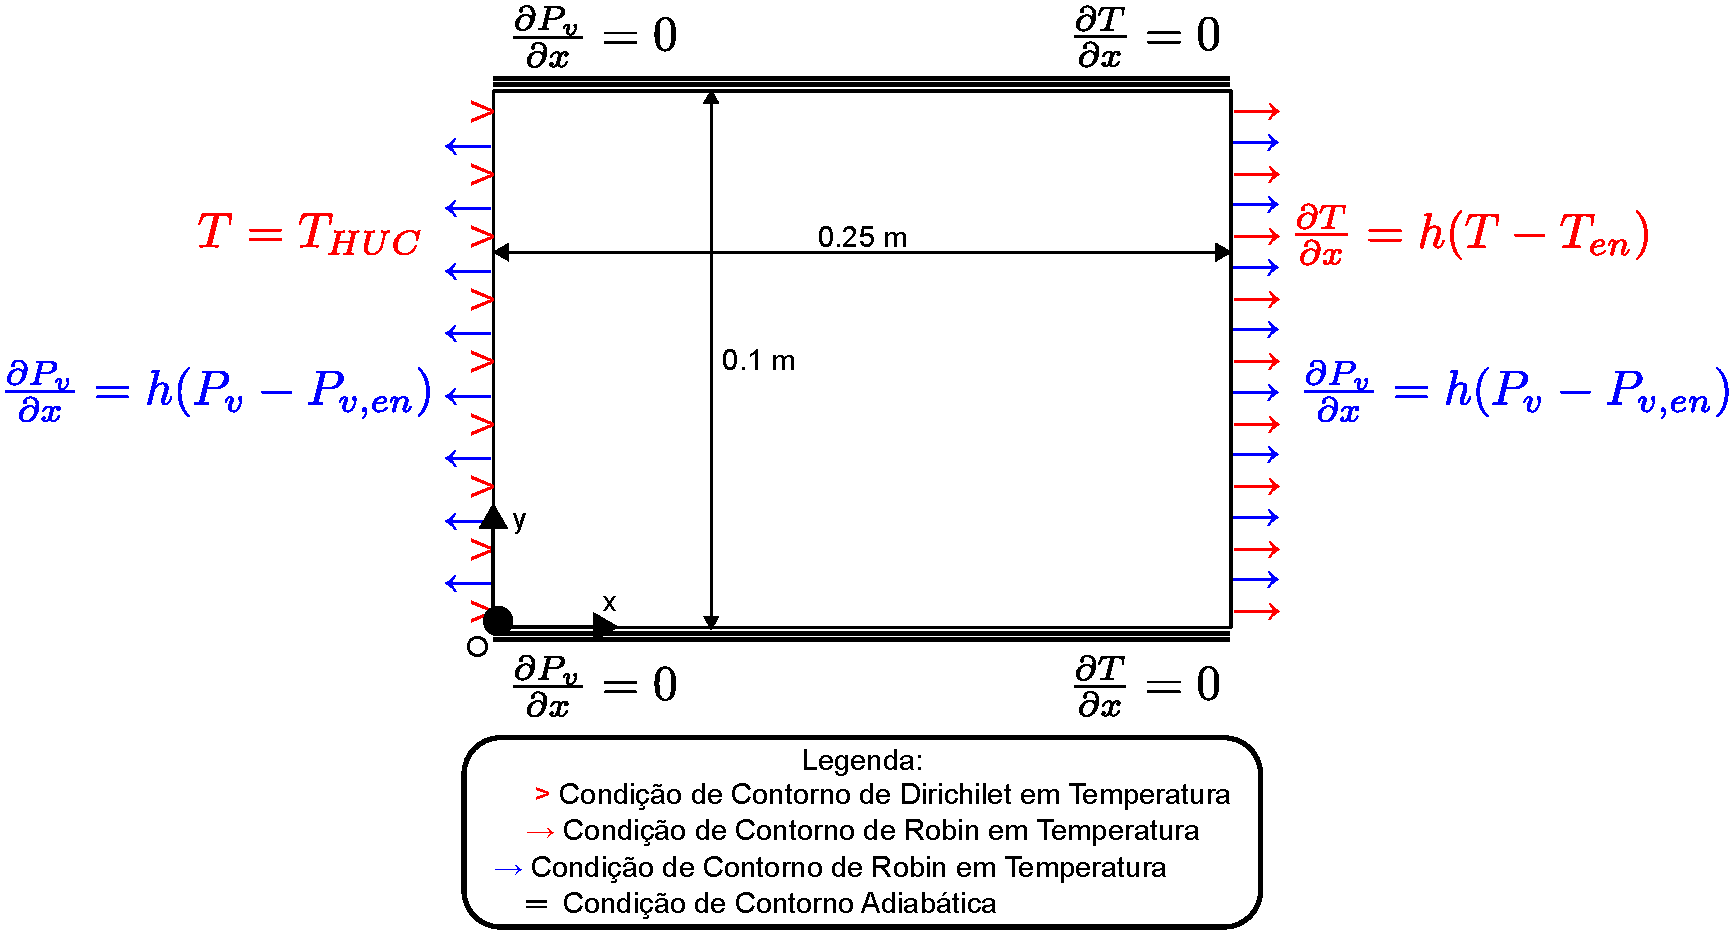
\includegraphics[width=14cm]{./figures/case.pdf}
	\caption{Esquema do caso ilustrativo apresentando as dimensões e condições de
    contorno aplicadas.  \label{fig:case}}
  \end{figure}

  \setlength{\tabcolsep}{38pt}
  
\begin{table}[]
\centering
\caption{Simulação do caso ilustrativo}
\label{tab:case_ics_bcs}
\addtolength{\tabcolsep}{-10pt}
\begin{tabular}{|ll|}
\hline
\multicolumn{2}{|l|}{Discretização no espaço e no tempo}                                    \\ \hline
Espessura da parede                                          & $L_x = 25 cm$                \\
Tempo simulado                                               & $t = 25 h$                   \\
Número de elementos em $x$                                   & $n_x = 50$                   \\
Número de elementos em $y$                                   & $n_y = 20$                   \\
Incremento de tempo                                          & $\Delta t = 15 s$            \\ \hline
\multicolumn{2}{|l|}{Condições Iniciais}                                                    \\ \hline
$T(x, y, t=0)$                                               & $ 25 ^{\circ}C$              \\
$P_v(x, y, t=0)$                                             & $ 2850 N \ m^{-2} $          \\ \hline
\multicolumn{2}{|l|}{Condições de Contorno}                                                 \\ \hline
$T(x=0, y, t)$                                               & $T_{HUC}(t)$                 \\
$\frac{\partial T}{\partial x}\bigg\rvert_{x = L_x, y, t}$   & $h \ (T - T_{en})$           \\
$\frac{\partial T}{\partial y}\bigg\rvert_{x, y=0, t}$       & $0$                          \\
$\frac{\partial T}{\partial y}\bigg\rvert_{x, y=L_y, t}$     & $0$                          \\
$\frac{\partial P_v}{\partial x}\bigg\rvert_{x = 0, y, t}$   & $h_m \ (P_v - P_{v, en})$    \\
$\frac{\partial P_v}{\partial x}\bigg\rvert_{x = L_x, y, t}$ & $h_m \ (P_v - P_{v, en})$    \\
$\frac{\partial P_v}{\partial y}\bigg\rvert_{x, y=0, t}$     & $0$                          \\
$\frac{\partial P_v}{\partial y}\bigg\rvert_{x, y=L_y, t}$   & $0$                          \\ \hline
\multicolumn{2}{|l|}{Propriedades}                                                          \\ \hline
Condutividade térmica do concreto refratário, $\lambda$      & $7 W \ m^{-1} \ K^{-1}$      \\
Densidade do concreto refratário, $\rho$                     & $2200 Kg \ m^{-3}$           \\
Calor específico do concreto refratário, $C_p$               & $1100 J \ Kg^{-1} \ K^{-1}$  \\
Curvas de Sorção Isotérmica, $w$                             & Equation \ref{eq:gong_phi}           \\
Permeabilidade, $K$                                          & Equation \ref{eq:baz_perm}           \\
Permeabilidade inicial, $K_0$                                & $ 10^{-12} m \ s^{-1}$       \\
Calor específico da água, $C_w$                              & $ 4100 J \ Kg^{-1} \ K^{-1}$ \\
Coeficiente de transferência de calor, $h$                   & $ 1 W \ m^{-2} \ K^{-1}$     \\
Coeficiente de transferência de calor, $h_m$                 & $ 1 \ 10^{-^6} s \ m^{-1}$   \\
Temperatura ambiente, $T_{en}$                               & $ 25 ^{\circ}C$              \\
Pressão Parcial de vapor de água, $P_{v, en}$                & $ 2850 N \ m^{-2} $          \\
Quantidade de cimento por Kg de concreto, $w_c$              & $ 300 Kg m^{-3} $            \\
Quantidade de água inicial por Kg de concreto, $w_0$         & $ 100 Kg m^{-3} $            \\ \hline
\end{tabular}
\end{table}

    A permeabilidade, ($K$), é retirada do modelo de Bažant, que também é utilizada pelo
    trabalho de Gong. Já a sorção isotérmica ($w$) é adaptada de \ref{eq:baz_phi}
    conforme descrito por Gong e representado pela Equação \ref{eq:gong_phi}.

\begin{equation}
  \label{eq:gong_phi}
      w(P, T) =
      \begin{cases} 
      w_c \left( \frac{w_0}{c} \ \phi(P,T) \right)^{\frac{1}{m(T)}} & \phi(P, T)\leq 0.96 \\
      w_{0.96} + (\phi(P, T) - 0.96) \frac{(w_{1.04} - w_{0.96})}{(1.04-0.96)} & 0.96 < \phi(P, T) < 1.04 \\
 w_c \ \left[0.037 (\phi-1.04) + 0.3335 \left(1 - \frac{T^2}{3.6 \ 10^5}) \right) \right] & \ 1.04 \leq \phi(P, T)
      \end{cases}
\end{equation}

    O uso de tal versão se justifica pois a equação é ajustada para a
    microestrutura de um concreto refratário \cite{Gong1995a} e ao não utilizar
    da porosidade, apresenta uma maior simplicidade de uso. Provido das
    propriedades apresentadas na Tabela \ref{tab:case_ics_bcs}, da geometria e
    das condições iniciais e de contorno, basta definir o sistema de equações a
    ser resolvido.

    \section{Sistema de Equações}\label{mat:eqs}
    Problemas de caráter transiente são modelos matemáticos cujas variáveis de
    resposta dependem do tempo. A solução de tais problemas através de modelos
    numéricos implica em uma discretização no tempo e no espaço. Há inúmeras
    estratégias para tal tarefa, porém no presente trabalho se utilizará de uma
    discretização espacial a partir de elementos finitos e temporal a partir de
    diferenças finitas.

    Conforme já apresentado na Seção \ref{sec:bazant}, a formulação se baseia no
    balanço de massa e energia dos fluxos de uma quantidade denominada umidade
    que representa tanto a água líquida livre, adsorvida e o vapor de água. A
    forma forte do sistema é composta pelas equações de balanço derivadas de
    \ref{eq:baz_MB} e \ref{eq:baz_EB}, pelas condições iniciais e de contorno. 
    
    \subsection{Forma Forte}\label{mat:forte}
    No presente modelo as variáveis independentes escolhidas são a temperatura
    $T$ e a pressão nos poros, $P_v$. A apresentação da formulação do problema em
    sua forma forte será descrito levando em consideração funções não explicítas
    das variaveis independentes a fim de simplificar as expressões matemáticas.

    
    Substituindo as Equações \ref{eq:Darcy}, \ref{eq:Fourier} nas
    Equações  \ref{eq:baz_MB} e \ref{eq:baz_EB} obtém-se o problema em sua forma
    forte:  

    Equações de Conservação:
   \begin{equation}
     \label{eq:full_MB}
     \frac{\partial w}{\partial t}  = \nabla \cdot \left(\frac{K}{g} \nabla P_v \right) + \frac{\partial w_d}{\partial t} \ \text{in } \Omega
   \end{equation}

   \begin{equation}
      \label{eq:full_EB}
      \frac{\partial T}{\partial t} = C_a \ \frac{\partial w}{\partial t} +  C_w \frac{K}{g} \ \nabla P_v \cdot \nabla T + \nabla \cdot (\lambda \nabla T) \ \text{in } \Omega
   \end{equation}

   Condição de contorno de Dirichlet:
   \begin{equation}
     \label{eq:dir_bc}
    T(0, y, t) = T_{HUC}(t) \ \text{in } \Gamma_D
   \end{equation}

   Condições de contorno de Neumann:
   \begin{equation}
     \label{eq:neu_bc_T_x}
     \frac{\partial T}{\partial x}\bigg\rvert_{x = L_x, y, t} =  (T - T_{en}) \ \text{in } \Gamma_{N, T_{env}}
   \end{equation}

   \begin{equation}
     \label{eq:neu_bc_T_y}
\frac{\partial T}{\partial y}\bigg\rvert_{x, y=0, t} = \frac{\partial T}{\partial y}\bigg\rvert_{x, y=L_y, t} = 0 \ \text{in } \Gamma_{N, adi}
   \end{equation}

   
   \begin{equation}
     \label{eq:neu_bc_P_x}
     \frac{\partial P_v}{\partial x}\bigg\rvert_{x = 0, y, t} = \frac{\partial P_v}{\partial x}\bigg\rvert_{x = L_x, y, t} =  h_m \ (P_v - P_{v, en}) \ \text{in } \Gamma_{N, P_{env}}
   \end{equation}

   \begin{equation}
     \label{eq:neu_bc_P_y}
    \frac{\partial P_v}{\partial y}\bigg\rvert_{x, y=0, t}= \frac{\partial P_v}{\partial y}\bigg\rvert_{x, y=L_y, t} = 0 \ \text{in }\Gamma_{N, adi}
   \end{equation}


   
    Deve-se salientar que as derivadas temporais das curvas de sorção são
    obtidas a seguir como função das derivadas parciais das variáveis
    independentes. Tal abordagem permite expressar o problema em termos mais simples.

    \begin{equation}
      \label{eq:dwdt}
      \frac{\partial w}{\partial t} = \frac{\partial w}{\partial P_v} \frac{\partial P_v}{\partial t} + \frac{\partial w}{\partial T} \frac{\partial T}{\partial t}
    \end{equation}

    Além disso, as derivadas temporais das variáveis independentes são aproximadas
    por diferenças finitas anteriores conforme descrito pelas Equações \ref{eq:fd_P} e \ref{eq:fd_T}.

    \begin{equation}
      \label{eq:fd_P}
      \frac{\partial P_v}{\partial t} = \frac{P_v - P_v^n}{\Delta t}
    \end{equation}
    
    \begin{equation}
      \label{eq:fd_T}
      \frac{\partial T}{\partial t} = \frac{T - T^n}{\Delta t}
    \end{equation}

    Por fim, as derivadas parciais das curvas de sorção isotérmica são
    aproximadas por diferenças finitas centrais, Equações \ref{eq:fc_P} e \ref{eq:fc_T}.

    \begin{equation}
      \label{eq:fc_P}
      \frac{\partial w}{\partial P_v^n} = \frac{w(P_v^n+\delta \ P_v^n, \ T^n)- w(P_v^n- \delta \ P_v^n , \ T^n)}{2 \ \delta}
    \end{equation}

    
    \begin{equation}
      \label{eq:fc_T}
      \frac{\partial w}{\partial T^n} = \frac{w(P_v^n, \ T^n+\delta \ T^n)- w(P_v^n, \ T^n- \delta \ T^n)}{2 \ \delta}
    \end{equation}

    Onde $\delta$ é um diferencial numérico com valor $\delta = 0.0001$.

    
    \subsection{Forma Fraca}\label{mat:fraca}
    A forma fraca é obtida a partir da multiplicação das equações de conservação
    de massa e de energia pela função teste $\psi$ e subsequente integração
    sobre o domínio numérico. É utilizada a identidade de Green quando aplicável
    para se obter a forma fraca final.

  \begin{equation}
     \label{eq:weak_MB}
  \int_{\Omega}  \frac{\partial w}{\partial t} \ \psi \ \text{d}x =   \int_{\Omega}    \frac{K}{g} \left(  \nabla P_v \cdot \nabla  \psi \right) \ \text{d}x +   \int_{\Omega}    \frac{\partial w_d}{\partial t}  \ \psi \ \text{d}S \ +   \int_{\Gamma_{N, P_{env}}} \left( P_v \cdot \mathbf{n} \right) \ \psi \ \text{in } \Omega
   \end{equation}

   \begin{eqnarray}
     \label{eq:weak_EB}
      \int_{\Omega} \frac{\partial T}{\partial t} \ \psi \ \text{d}x &=&
                                                                         \int_{\Omega}
                                                                         C_a \
                                                                         \frac{\partial
                                                                         w}{\partial
                                                                         t} \
                                                                         \psi \
                                                                         \text{d}x
                                                                         +
                                                                         \int_{\Omega}
                                                                         C_w
                                                                         \frac{K}{g}
                                                                         \
                                                                         \nabla
                                                                         P_v
                                                                         \cdot
                                                                         \nabla
                                                                         T \
                                                                         \psi \
                                                                         \text{d}x
     \nonumber \\
                                                                         & &+ \int_{\Omega} \lambda \ \nabla T \cdot \nabla \psi \ \text{d}x + \int_{\Gamma_{T_{env}}} \left( T \cdot \mathbf{n} \right) \ \psi \ \text{d}x \ \text{in } \Omega
    \end{eqnarray}

    
    Tal sistema é fornecido à biblioteca FEniCS que converte o sistema de
    equações parciais diferenciais em um sistema linear de equações baseado nas
    funções de forma escolhidas. Esse sistema é resolvido iterativamente e o
    resultado é obtido através dos valores nodais (em cada um dos nós da malha
    que representa a discretização da geometria do problema) das variáveis de interesse.

    A seguir será delineado a estrutura do código apresentando uma clara
     correlação com cada etapa da descrição matemática.
     
    \section{Estrutura do script}\label{mat:script}
    O script pode ser separado nas seguintes etapas:

    \begin{itemize}
    \item Importação das bibliotecas necessárias
    \item Definição dos parâmetros de discretização temporal e espacial
    \item Definição da malha a partir da geometria
    \item Especificação das condições de contorno
    \item Definição dos espaços das funções de elementos finitos
    \item Definição das propriedades dos materiais
    \item Especificação das condições iniciais
    \item Descrição do sistema de equações em sua forma fraca
    \item Loop temporal de resolução das equações e armazenamento dos resultados 
    \end{itemize}

    Cada uma das etapas serão detalhadas e o código mostrado.

    
    \subsection{Importação das bibliotecas}
    Para a simulação, apenas o pacote \mintinline[bgcolor=bg]{python}{dolfin} da biblioteca
    FEniCS é necessário. O pacote \mintinline[bgcolor=bg]{python}{datetime} é utilizado para
    contabilizar o tempo decorrido de simulação. Já os pacotes
    \mintinline[bgcolor=bg]{python}{csv} e \mintinline[bgcolor=bg]{python}{os} são importados para
    salvar as séries temporais de variáveis de interesse em uma planilha e para 
    gerenciar em qual diretório serão salvos os arquivos, respectivamente.

    \begin{minted}[
      frame=lines,
      framesep=2mm,
      baselinestretch=1.2,
      bgcolor=bg,
      fontsize=\footnotesize,
      linenos
      ]{python}

      from dolfin import *
      from datetime import datetime
      import csv
      import os
    \end{minted}
   
    \subsection{Definição da discretização}
    Conforme definido na Tabela \ref{tab:case_ics_bcs}, a discretização é
    definida a partir das seguintes variáveis.
    
    \begin{minted}[
      frame=lines,
      framesep=2mm,
      baselinestretch=1.2,
      bgcolor=bg,
      fontsize=\footnotesize,
      linenos
      ]{python}
      
      # Time discretization
      t = 0
      T_total = 25 * 3600
      dt = 15
      
      # Space discretization
      lx = 0.25
      ly = 0.10
      Nx = 50
      Ny = 20
    \end{minted} 

    \subsection{Definição da malha e das condições de contorno}
    O pacote FEniCS já vem com uma ferramenta capaz de gerar malhas em
    geometrias simplistas. Dessa forma, para definir a malha da seção retangular
    da parede do caso de estudo é simples utilizando apenas a função
    \mintinline[bgcolor=bg]{python}{RectangleMesh()}. Em seguida, cria-se um
    objeto que representa as condições de contorno através da função
    \mintinline[bgcolor=bg]{python}{MeshFunction()}, cujos argumentos definem
    qual o tipo desse contorno (face interna ou externa), a malha, e a dimensão
    do contorno (pontos para um domínio unidimensional, curvas para domínios
    bidimensionais e superfícies para domínios tridimensionais). Por fim, é
    criada uma classe para cada parede do retângulo. Tais classes são utilizadas
    para marcar uma bandeira em cada nó que pertence a tais contornos. Por fim é
    criada uma medida através da função \mintinline[bgcolor=bg]{python}{Measure()} que será utilizada na formulação da forma fraca.
    
    \begin{minted}[
      frame=lines,
      framesep=2mm,
      baselinestretch=1.2,
      bgcolor=bg,
      fontsize=\footnotesize,
      linenos
      ]{python}

      # Mesh and Boundaries Condition Definitions
      mesh = RectangleMesh(0.0, 0.0, lx, ly, Nx, Ny)

      # Boundaries
      boundaries = MeshFunction('size_t', mesh, mesh.topology().dim() - 1)
      boundaries.set_all(0)


      class left(SubDomain):
          def inside(self, x, on_boundary):
              return abs(x[0]) < DOLFIN_EPS and on_boundary
      

      class right(SubDomain):
          def inside(self, x, on_boundary):
              return abs(x[0] - lx) < DOLFIN_EPS and on_boundary


      class top(SubDomain):
          def inside(self, x, on_boundary):
              return abs(x[1] - ly) < DOLFIN_EPS and on_boundary


      class down(SubDomain):
          def inside(self, x, on_boundary):
              return abs(x[1]) < DOLFIN_EPS and on_boundary


      left = left()
      right = right()
      top = top()
      down = down()
      left.mark(boundaries, 1)
      right.mark(boundaries, 2)
      top.mark(boundaries, 3)
      down.mark(boundaries, 4)
      ds = Measure("ds", domain=mesh, subdomain_data=boundaries)
    \end{minted} 

    \subsection{Definição dos espaços das funções de elementos finitos}
    Uma vez definida as geometrias do problema, criam-se o espaço da função de
    elementos finitos onde residem as funções teste e as funções bases que
    aproximação as variáveis independentes do problema (a temperatura e a
    pressão). Como o problema é acoplado de maneira forte, o espaço vetorial
    deverá compreender elementos que aproximem ambas as funções e para tanto
    cria-se um espaço misto. Para tanto, é criado primeiramente um objeto que
    representa um elemento finito linear
    \mintinline[bgcolor=bg]{python}{RectangleMesh(P1)}. Em seguida define-se o
    elemento misto e o espaço de função sobre a malha usando a
    função\mintinline[bgcolor=bg]{python}{FunctionSpace()}. A partir daí é
    possível obter funções teste e funções de aproximação a partir do espaço V.  
    
     \begin{minted}[
      frame=lines,
      framesep=2mm,
      baselinestretch=1.2,
      bgcolor=bg,
      fontsize=\footnotesize,
      linenos
      ]{python}
     # Mixed element and space functions definition
     P1 = FiniteElement('P', mesh.ufl_cell(), 1)
     element = MixedElement([P1, P1])
     V = FunctionSpace(mesh, element)
     v_1, v_2 = TestFunctions(V)
     u = Function(V)
     P_v, T = split(u)
     u_n = Function(V)
     P_v_n, T_n = split(u_n)

    \end{minted} 
   
    \subsection{Definição das propriedades do material}
    Cada uma das propriedades são definidas através de funções definidas em
    python. A única especificidade referente ao uso da plataforma FEniCS é o uso
    de uma função própria para definir condicionais. 

    \subsection{Especificação das condições iniciais}
    As condições iniciais são projetadas no espaço de elementos finitos usando a
    função \mintinline[bgcolor=bg]{python}{interpolate()}.
    
    \begin{minted}[
      frame=lines,
      framesep=2mm,
      baselinestretch=1.2,
      bgcolor=bg,
      fontsize=\footnotesize,
      linenos
      ]{python}
     
     # Initial conditions
     P_0 = P_v_inf
     P_v_n = interpolate(P_0, V.sub(0).collapse())
     T_0 = Constant(298.15)
     T_n = interpolate(T_0, V.sub(1).collapse())
    \end{minted} 

    \subsection{Descrição da forma fraca}
    Em seguida, a forma fraca é definida. Na presente subseção também será
    criado um objeto que representa o problema numérico a ser resolvido.
    A representação é direta do problema descrito em \ref{mat:fraca}. A
    integração é apenas representada implicitamente pela
    multiplicação de cada termo pela medida volumétrica
    \mintinline[bgcolor=bg]{python}{dx} ou de contorno
    \mintinline[bgcolor=bg]{python}{ds}.

    Também se define o Jacobiano do resíduo que será utilizado no algoritmo de
    resolução através do método de Newton. Por fim, são definidos objetos que
    representam o problema numérico (\mintinline[bgcolor=bg]{python}{problem}) e o algoritmo de solução em si (\mintinline[bgcolor=bg]{python}{solver}).
    
    \begin{minted}[
      frame=lines,
      framesep=2mm,
      baselinestretch=1.2,
      bgcolor=bg,
      fontsize=\footnotesize,
      linenos
      ]{python}

     # Variational formulation in residual form
     # Mass balance equation equation
     ResP = dwdt(P_v, T, P_v_n, T_n) * v_1 * dx
     ResP += (a(P_v_n, T_n) / g) * inner(nabla_grad(P_v), nabla_grad(v_1)) * dx
     ResP += - ((w_d(T) - w_d(T_n)) / dt) * v_1 * dx
     ResP += B_w * (P_v - P_v_inf) * v_1 * (ds(1) + ds(2) + ds(3) + ds(4))


     # Energy balance equation
     ResT = rho * C_p * ((T - T_n) / dt) * v_2 * dx
     ResT += k * inner(nabla_grad(T), nabla_grad(v_2)) * dx
     ResT += - h_d * ((w_d(T) - w_d(T_n)) / dt) * v_2 * dx
     ResT += - C_a(T_n) * dwdt(P_v, T, P_v_n, T_n) * v_2 * dx
     ResT += C_w * (a(P_v_n, T_n) / g) * \
         inner(nabla_grad(P_v_n), nabla_grad(T_n)) * v_2 * dx
     ResT = ResT + (B_t * (T - T_inf) +
                   C_a(T_n) * B_w * (P_v - P_v_inf)) * v_2 * (ds(2) + ds(3))


     # Total residual
     Res = ResT + ResP

     # Jacobian
     Jac = derivative(Res, u)
     problem = NonlinearVariationalProblem(Res, u, bcs, Jac, ffc_options)
     solver = NonlinearVariationalSolver(problem)
    \end{minted} 

    \subsection{Loop temporal}
    Em seguida, após a definição do problema e do objeto que representa o
    algoritmo de solução cria-se um loop que deverá rodar até o tempo de
    simulação alcançar o tempo total simulado (25 h). A evolução da pressão
    máxima, da temperatura máxima e da quantidade de água livre do sistema são
    salvos em um arquivo .csv que permite sua visualização online (i.e. durante
    a simulação).

    Ao entrar no loop o tempo atual de simulação é utilizado para
    definir em qual etapa da curva de aquecimento se está. Isto define a
    temperatura na condição de contorno de Dirichlet. Em seguida é resolvido o
    sistema linear de equações. A quantidade de água livre no sistema é
    integrada ao longo do domínio e os valores do timestep anterior são
    igualados ao timestep atual. A cada dez ciclos dentro do loop os resultados
    de todo o domínio são salvos em um arquivo que pode ser visualizado através
    da plataforma Paraview \cite{paraview2007}. O tempo de simulação é corrigido e o ciclo se
    inicia novamente.

    Ao alcançar o tempo total de simulação o programa saí do loop, o arquivo csv
    é salvo e se calcula o tempo real gasto pela simulação.
    
     \begin{minted}[
      frame=lines,
      framesep=2mm,
      baselinestretch=1.2,
      bgcolor=bg,
      fontsize=\footnotesize,
      linenos
      ]{python}
     f = open(dir_ + '/time_series.csv', 'w')
     writer = csv.writer(f, delimiter='\t')
     startTime = datetime.now()
     while t <= T_total:

         print('Progress: ' + str(round(t / T_total * 100, 2)) + '%')
     
         # Solve non-linear problem
         T_huc.t = t
         if t < 5 * 3600:
             T_huc.rate = 50
             T_huc.T_0 = 298.15
         elif (t > 5 * 3600) & (t < 10 * 3600):
             T_huc.rate = 0
             T_huc.T_0 = 298.15 + 250
         elif (t > 10 * 3600):
             T_huc.rate = 30
             T_huc.t_0 = 15.833 * 3600
             T_huc.T_0 = 298.15 + 250

         n, conv = solver.solve()

         # integration over domain of water quantity
         wat = assemble((w(P_v_n, T_n)) * dx,
                        form_compiler_parameters=ffc_options)
         w_domain.append(wat)
         convergence.append(n)
         time.append(t)

         # Update solution with last computed value
         (_P, _T) = u.split(True)
         P_v_n.vector()[:] = _P.vector()
         T_n.vector()[:] = _T.vector()
         P_v_max = max(P_v_n.vector()[:]) / 1e6
         P_v_min = min(P_v_n.vector()[:]) / 1e6
         T_max = max(T_n.vector()[:])
         T_min = min(T_n.vector()[:])

         writer.writerow([t, H, wat, n, T_max, P_v_max])

         if (nt % freq_out == 0):
             _P.rename("Pressure [Pa]", "P_v")
             _T.rename("Temperature [K]", "T")
             filex.write(_P, t)
             filex.write(_T, t)

         nt += 1
         t += dt
     # End loop over time steps
     f.close()
     time_delta = datetime.now() - startTime
     print('Simulation time: ', str(time_delta))
    \end{minted} 
   
    \section{Pós-processamento}
    O pós processamento se dá através de dois tipos de dados principais, são
    eles o arquivo csv que tem como objetivo dar um indicativo qualitativo da
    convergência correta da simulação (isto é, se o resultado é condizente, se a
    temperatura de aquecimento é obedecida, se a pressão máxima é um valor
    coerente ou se a quantidade de água está seguindo o comportamento já
    esperdo), e os dados nodais de todo o domínio.

    Os dados do domínio são os mais importantes porém resultam em arquivos
    pesados (dependendo do refinamento da malha e do tamanho do incremento de
    tempo). Portanto dependendo da simulação o intervalo de registro dos dados
    pode ser maior ou menor. Análises qualitativas são realizadas usando o
    Paraview enquanto análises quantitativas, descritas em termos de gráficos da
    evolução de propriedade em diferentes posições ou de perfis térmicos em
    diferentes tempos, são obtidos por rotinas em Python.





\end{apendicesenv}
% ---


% ----------------------------------------------------------
% Anexos
% ----------------------------------------------------------

% ---
% Inicia os anexos
% ---
\begin{anexosenv}

\chapter{Anexo} \label{orcamento}

%\includepdf[pages=1-2]{DFA100.pdf}

\end{anexosenv}

%---------------------------------------------------------------------
% INDICE REMISSIVO
%---------------------------------------------------------------------

\printindex

\end{document}
